\documentclass[11pt]{article}
%%%%%%%%%%%%%%%%%%%%%%%%%%%%%%%%%%%%%%%%%%%%%%%%%%%%%%%%%%%%%%%%%%%%%%%%%%%%%%%
% Packages, Commands and Miscellaneous
%%%%%%%%%%%%%%%%%%%%%%%%%%%%%%%%%%%%%%%%%%%%%%%%%%%%%%%%%%%%%%%%%%%%%%%%%%%%%%%

%%%=== PART 1: Packages
\usepackage{amsfonts, amsmath, amssymb}
\usepackage[toc,page]{appendix}
\usepackage{bbm}                              %% for indicator function notation
\usepackage{enumitem}                         %% for customising bullet point lists
\usepackage{float, graphicx, svg, subcaption}
\usepackage{hyperref}                         %% for in-document references
\usepackage[utf8]{inputenc}                   %% for compiler to interpret .tex file
\usepackage{setspace}                         %% for setting vspace between sentences
\usepackage{tikz}                             %% for drawing Bayesian networks
\usepackage{tcolorbox}
\usepackage{xcolor}

\usepackage[pass]{geometry} %% for the minimisation of margins
\newlength\DX
\DX=3.0in
\paperwidth=\dimexpr\paperwidth-\DX\relax
\hoffset=\dimexpr\hoffset-.5\DX\relax
\newlength\DY
\DY=2.8in
\paperheight=\dimexpr\paperheight-\DY\relax
\voffset=\dimexpr\voffset-.5\DY-.5\footskip\relax

%%%=== PART 2: Commands
\newcommand{\D}{\mathcal{D}}
\newcommand{\E}{\mathbb{E}}
\newcommand{\R}{\mathbb{R}}
\newcommand{\X}{\mathbf{X}}
\newcommand{\Z}{\mathbf{Z}}

\newcommand{\x}{\mathbf{x}}
\newcommand{\z}{\mathbf{z}}

\newcommand{\REVIEW}{\textcolor{purple}{\textbf{REVIEW: }}}
\newcommand{\TODO}{\textcolor{red}{\textbf{TODO: }}}
\newcommand{\IMPROVE}{\textcolor{myYellow}{\textbf{IMPROVE: }}}

\renewcommand{\l}{\left}
\renewcommand{\r}{\right}

%%%=== PART 3: Miscellaneous
\captionsetup{labelfont=bf}

\DeclareMathOperator*{\argmax}{arg\,max}
\DeclareMathOperator*{\argmin}{arg\,min}

\definecolor{myDarkBlue} {RGB}{ 15, 61,138}
\definecolor{myGreen}    {RGB}{  0,128,128}
\definecolor{myLightBlue}{RGB}{173,216,230}
\definecolor{myLightRed} {RGB}{255, 99, 71}
\definecolor{myYellow}   {RGB}{255,165,  0}


\begin{document}

% title
\begin{center}
\HRule\\[0.6cm]
{\huge\bfseries Machine Learning Explainers}\\[0.2cm]
\textbf{Last updated:} \today\\
\HRule\\[0.6cm]
\end{center}

% abstract
\begin{abstract}
    \noindent Summaries of a bunch of machine learning-related topics. My main motive in writing these summaries is as a reminder for my future self.
\end{abstract}

% table of contents
\setcounter{tocdepth}{2}{\small\tableofcontents}

% intro
\section{Introduction}

I personally think of machine learning as modelling the relationship between model variables $\X$ and output variables $\Y$, be the relationship probabilistic or not, in line with the demands of the task to be solved. Vaguely put, this is done by constructing some parameterized representation $f_{\theta}$ of their relationship. Some parameters do a better job than others, according to some metric of goodness, so we'd ideally have the optimal parameters $\theta^{*}$.

What makes machine learning fun is that, for whatever reason, these learned representations of underlying relationships can be used to infer things about the relationship of $\X$ and $\Y$ very well. The fact that this is possible to at least a small extent isn't too surprising, but, nowadays, this is possible to the extent of being able to do things like input natural language to output a photo-realistic image described by said input. Why is this possible? The more I've learned, the more I'm amazed that our methods work as well as they do. Take denoising diffusion models for image generation. It effectively learns to transform randomly sampled Gaussian noise into something convincingly belonging to the distribution pertainintg to the data that the model was trained on. So if I train such a model on a large dataset of images of cats then it learns to transform Gaussian noise into new images of cats that are sufficiently distinct from those it was trained on. That is, such models do not necessarily need to overfit to be able to output samples convincingly belonging to the target distribution. Why are diffusion, flow-based models, GANs, VAEs, probabilistic circuits or attention-based models so effective? It's sometimes hard to believe, even after working with some of these architectures extensively and understanding them in detail.

% thoughts on reasoning
\section*{Thoughts on `reasoning'}

As a term, machine learning is used almost interchangeably with AI as of now (summer of 2024). AI isn't particularly well-defined in itself, even in academic settings, so its use in day-to-day things, like the news, can be confusing. I think of machine learning as what's written above, effectively in line with statistical learning theory. I'm not sure how I would define AI in a way that'd satisfy most. Maybe the discipline of studying things that can `reason', as a human does, given some agreeable notion of `reasoning'. A common issue found in discussions surrounding this topic is that a definition of `reasoning' is left out. In fairness, it's a tricky thing to define precisely. For a long time, people considered the Turing test to be a metric in line with the idea of machines `reasoning'. Current LLMs are far beyond passing the Turing test but still it is argued that they don't reason, which I think I agree with as of now, but it's worth being conscious of the fact that we have effectively moved the goal posts. A similar example of this is the Automatic Statistician: a model that, given a bunch of data, can effectively output a report on the likely relationships between different parts of the data\footnote{\url{https://www.youtube.com/watch?v=aPDOZfu_Fyk}}. Essentially a data scientist or statistician in the form of a machine, which we're much closer to than in say 2020 due to LLMs.

Right now, I'm unaware of any machine learning model that can `reason' by any agreeable notion of the term. Let's say that GPT-4o concludes that a continuous real-valued function $f:\R\rightarrow\R$ has a root in some interval $(a, b)$ using the intermediate value theorem (IVT) by noting that $f(a)<0$ and $f(b)>0$. Is this `reasoning' or do we instead brush this off as the model having been trained on a bunch of examples of the use of IVT? Does it understand what it's concluding? As of right now I'd say that it doesn't. This of course isn't something unique to IVT - we can construct many such examples. What I think makes IVT interesting is that we can effectively express what it means to understand it as a human. I'd say that the distinction between ChatGPT's `understanding' here and a human's is that a human knows that if they trace their finger on a piece of paper starting from the bottom half, crossing a horizontal line cutting through the middle, to the top half of the page without taking their finger off the paper then their finger must have touched the horizontal line at some point, i.e. the function must have intersected the $x$-axis during this continuous traversal. I believe that humans understand this due to just experiencing the real world. You don't need any mathematical training to know and, more importantly, understand `why' your finger crosses through this horizontal line on the page. I'm certain that current GPT models do not `understand' the IVT in this way, or really any way that isn't purely formally mathematical.

A follow up question is to what extent it matters that a model `understands' how it arrives at its conclusions. Somewhat in the same way that it doesn't matter that a calculator has no inherent idea of why it outputs 6 when you input $3\cdot2$. Maybe 50 years from now we'll be well-taken care of by a fleet of machine learning-based robots and we'll still complain that they aren't truly capable of reasoning like us. Hopefully not. I wish industry research in certain areas of machine learning, like LLMs and image/video generation, would be very heavily regulated. Perhaps forcefully stopped entirely. Of course, this will never happen due to countries' desire to be ahead of their competitors.

% misc.
Some things I've heard prominent figures in AI say that gelled with me:
\begin{itemize}
    \item Allan Newell: know what you're bad at! (add source youtube vid)
    \item Marvin Minsky: when I get to the point that I understand something or have successfully implemented something it no longer seems difficult. In fact, there's thing feeling of it never having \textit{really} been difficult. I don't like this since it takes away that feeling of self-reward of ``well done Dewi you did something''.
    \item Stuart Russell: similar comment to his ``it's as if Aliens came down and gave us this deep learning technology''
\end{itemize}

% supervised learning
\section{Supervised Learning}

Supervised learning algorithms are a class of machine learning algorithms in which a model learns some relationship between model variables and output variables by being shown concrete examples of what a given input (pertaining to the model variables) should yield as output. These model and output variables can be continuous or discrete in nature but usually it's a mix.

An example of a task which supervised learning is appropriate for includes regression predicting life expectancies of a poulation given features such as the population's height, age, BMI etc. You can think of regression tasks as those where the output of the model should belong to some continuously distributed space. Other than regression, the other vanilla supervised learning task is binary or multi-class classification. Well known examples of binary classification include whether or not a given passenger survived the titanic wreck given their ticket class, sex, age, port of embarkation and a ton more. The bread and butter example of multi-class classification is handwritten digit recognition. It's amazing that something difficult as recently as 2005 is trivial now for various levels of machine learing understanding.

Other than the types of tasks which we consider in this section, it's worth mentioning how we deal with our data in general. In training a model on some dataset, we need some idea of how well the model generalises to new data. This is done by splitting the given dataset $\D$ into a training set $\Dtrain$ and a testing set $\Dtest$. How exactly this split is done depends on the task at hand but an example is 50/50 uniformly randomly splitting the original dataset $\D$ - chronologically or not. It can be important that this is done uniformly randomly. For example, if one is tackling a binary classification task and $\D$ consists of $1000$ samples with $500$ belonging to class 1 and $500$ belonging to class 2 then it's important that one does not split in a way that causes egregiously imbalanced representations of these classes. Training a model on $500$ samples of class 1 then testing it on $500$ samples of class 2 wouldn't make much sense. Similar idea for regression tasks but with ensuring a reasonable balance in representation of values belonging to given intervals corresponding to the output space. With a reasonable split we train the model on $\Dtrain$. It is all the model knows - $\Dtrain$ is the model's universe. After training, we measure the model's ability to generalise to new samples belonging to the same underlying distribution by seeing how well it performs with respect to the samples in $\Dtest$. Essentially comparing its output given some sample to the ideal/true output value of said sample. Things get a bit more fancy when we consider cross-validation but that'll come later.

% linear regression
\subsection{Linear Regression}

\textbf{Note:} There are some pieces of literature that define linear regression models as regression models that are linear in their parameters. By this definition, linear regression, as a term, would encompass polynomial regression models and other regression models with non-linear basis functions so long as the model is linear in its parameters. This confuses me as `linear regression' most often refers to models that fit a hyperplane to the data.

In fairness, from what I understand, using the least squares method derived below for all such regression models linear in their parameters is viable.\\

\noindent Perhaps the simplest example of supervised learning is linear regression. Suppose we are given a dataset $\D=\{(\x_i,y_i)\}_{i=1,\dots,2n}$ where
$$
\x_i=(x_{i,1},\dots,x_{i, p})\in \Omega_{X_1}\times\dots\times \Omega_{X_p}=:\OX\subseteq\R^p
$$
are the feature values of the $i^{\text{th}}$ sample and $y_i\in \OY\subseteq\R$ is the corresponding output. The reason I chose $|\D|=2n$ is that it results in being able to 50/50 split $\D$ into $\Dtrain$ and $\Dtest$ with $|\Dtrain|=|\Dtest|=n$. A linear regression models fits a linear function (in the parameters)
\begin{align*}
    f_{\theta}:\OX&\rightarrow \Omega_Y\\
    \x&\mapsto
    \theta^{\T}
    \begin{bmatrix}
        1\\
        \x
    \end{bmatrix}
    =
    \theta_0+\theta_1x_1+\dots+\theta_px_p    
\end{align*}
where $\theta=(\theta_0,\theta_1\dots,\theta_p)\in\R^{p+1}$ are the model parameters, i.e. the values we can tweak to our heart's desire until the corresponding model is sufficiently well according to some metric. Some people refer to the paramter $\theta_0$, which dictates the elevation of the hyperplane corresponding to $f_{\theta}(\x)=0$, as the bias of the model which I find very confusing as there are a bunch of other intended meanings of the term `bias' in statistics and machine learning. I prefer to refer to it as the elevation. Anyway, once such a linear function has been fit, given feature values $\tilde{\x}\in\OX$ we can predict the corresponding output as $\tilde{y}=f_{\theta}(\tilde{\x})$.

An intuitive approach to finding the `optimal' parameters for a linear regression model, which we denote by $\thetaOpt$, is to split $\D$ into training and testing datasets $\Dtrain$ and $\Dtest$ (each consisting of $n$ sample in our case) and minimising some pre-determined loss function of said parameters over $\Dtrain$. Essentially, minimising something like
$$
\text{Loss}(\theta)=\sum_{i=1}^nd(f_{\theta}(\x_i), y_i)
$$
where $f_{\theta}(\x_i)$ is the model's prediction for feature values $\x_i$ and $d:Y\times Y\rightarrow\R_{\geq0}$ is some metric on the set of possible output values and itself. Said loss function gives one an idea of how well $\theta$ fits the true underlying relationship which we wish to model. A common choice for the loss function is the mean square error
$$
\text{MSE}(\theta)=\sum_{i=1}^n(y_i-f_{\theta}(\x_i))^2
$$
which pertains to taking $d(f_{\theta}(\x_i), y_i)=(y_i-f_{\theta}(\x_i))^2$. I'll still refer to it as the `mean' square error, even though I don't divide by $n$, simply because minimising it as written above is equivalent to minimising the same expression with division by $n$ included - it's mostly a notational convenience thing. So in our case, we wish to find
$$
\thetaOpt=\argmin_{\theta\in\R^{p+1}}\left[\sum_{i=1}^n(y_i-f_{\theta}(\x_i))^2\right].
$$

\noindent We know that in the context of linear regression, the optimal paramters $\thetaOpt$ are typically taken to be those which minimise the mean square error over $\Dtrain$ but how do we actually compute $\thetaOpt$? This could be done through numerical methods, which is often the case in machine learning, e.g. using gradient descent in computing the optimal parameters of a logistic regression model, but linear regression has a closed form solution. This is pretty cool since it's not so common for such closed form solutions to exist. The informal method which I use to remember the closed form solution for the optimal paramters of a linear regression model is
$$
X\thetaOpt=y \implies X^{\T}X\thetaOpt=X^{\T}y \implies \thetaOpt=(X^{\T}X)^{-1}X^{\T}y.
$$
In practice, if this matrix $X^{\T}X$ is singular then just add some small values to its diagonal. That is, instead compute
$$
\thetaOpt=(X^{\T}X+\delta I)^{-1}X^{\T}y
$$
for some small $\delta\in\R$. That said, what's given above is not rigorous, so let's derive it. Note that
\begin{align*}
    \text{MSE}(\theta)
    &=
    \sum_{i=1}^n(y_i-f_{\theta}(\x_i))^2\\
    &=
    \begin{bmatrix}
        y_1-f_{\theta}(\x_1) & \cdots & y_n-f_{\theta}(\x_n)
    \end{bmatrix}
    \begin{bmatrix}
        y_1-f_{\theta}(\x_1)\\
        \vdots\\
        y_n-f_{\theta}(\x_n)
    \end{bmatrix}\\
    &=(y-X\theta)^{\T}(y-X\theta)\\
    &=||y-X\theta||^2
\end{align*}
where
$$
y
=
\begin{bmatrix}
    y_1\\
    \vdots\\
    y_n
\end{bmatrix}
\in\R^n,
X
=
\begin{bmatrix}
    1 & x_{1,1} & \cdots & x_{1,p}\\
    \vdots & \vdots & \ddots & \vdots\\
    1 & x_{n,1} & \cdots & x_{n,p}
\end{bmatrix}
\in\R^{n\times (p+1)},
\theta
=
\begin{bmatrix}
    \theta_0\\
    \theta_1\\
    \vdots\\
    \theta_p
\end{bmatrix}
\in\R^{p+1}
$$
and $x_{i,j}$ denotes the $j$th element of the $i^{\text{th}}$ sample. To find the minimiser(s) of $\text{MSE}(\theta)$, i.e. the optimal parameters $\thetaOpt$, we compute its gradient with respect to $\theta$, set it to $0$ and solve for $\thetaOpt$. This of course only works when our function is both differentiable and convex, which is the case here. To see convexity, simply compute the Hessian of $\text{MSE}(\theta)$ and see that it is semi-positive definite. On that note, we have
\begin{align*}
    \nabla\text{MSE}(\theta)
    &=
    \nabla||y-X\theta||^2\\
    &=
    \nabla(y-X\theta)^{\T}(y-X\theta)\\
    &=
    \nabla\left[\theta^{\T}X^{\T}X\theta-\theta^{\T}X^{\T}y-y^{\T}X\theta+y^{\T}y\right]\\
    &=
    \nabla\left[\theta^{\T}X^{\T}X\theta-2y^{\T}X\theta+y^{\T}y\right]\\
    &=
    2X^{\T}X\theta-2X^{\T}y
\end{align*}
and so the optimiser $\thetaOpt$ is given by
$$
\thetaOpt=(X^{\T}X)^{-1}X^{\T}y.
$$

\subsubsection{Statistical Motivation}

This idea of minimising the mean square error of the model over $\Dtrain$ even has some rigorous statistical motivation. Assume that the residuals corresponding of the model's output over $\Dtrain$ are independent and identically normally distributed with mean 0. That is, assume $e_i=y_i-f_{\theta}(\x_i)\sim\N(0, \sigma^2)$ for $i=1,\dots,n$ are i.i.d. This assumption is reasonable in practice via the CLT. Since $f_{\theta}(\x_i)$ is a constant, we have $y_i|\x_i\sim\N(f_{\theta}(\x_i), \sigma^2)$ and so
$$
\P(y_i|\x_i;\theta)=\frac{1}{\sqrt{2\pi}\sigma}\exp\left(-\frac{(y_i-f_{\theta}(\x_i))^2}{2\sigma^2}\right).
$$
By the law of maximum likelihood\footnote{maximum likelihood link}, the maximum likelihood estimator $\theta_{\text{MLE}}$ for the parameters of our linear regression model is that which maximise our log-likelihood. That is,
\begin{align*}
    \theta_{\text{MLE}}&=\argmax_{\theta}\left[\log\left(\prod_{i=1}^n\P(y_i|\x_i;\theta)\right)\right]\\
    &=\argmax_{\theta}\left[\sum_{i=1}^n\log(\P(y_i|\x_i;\theta))\right]\\
    &=\argmax_{\theta}\left[n\log\left(\frac{1}{\sqrt{2\pi}\sigma}\right)-\frac{1}{2\sigma^2}\sum_{i=1}^n(y_i-f_{\w,b}(\x_i))^2\right]\\
    &=\argmin_{\theta}\left[\sum_{i=1}^n(y_i-f_{\w,b}(\x_i))^2\right].
\end{align*}
As such, the maximum likelihood estimator of the parameters of a linear regression model are precisely those which minimise the mean square error of the model over $\Dtrain$.

\subsubsection{Example}

\begin{table}[ht]
    \begin{center}
        \begin{tabular}{c|c||c}
            Age (years) & BMI (kg/m$^2$) & Cholesterol (mg/dL)\\
            \hline
            \hline
            25 & 22.5 & 180 \\
            30 & 24.0 & 190 \\
            35 & 26.5 & 210 \\
            40 & 28.0 & 220 \\
            45 & 29.5 & 240 \\
            50 & 30.0 & 250 \\
            55 & 31.5 & 260 \\
            60 & 32.0 & 270 \\
            65 & 33.5 & 280 \\
            70 & 34.0 & 290 \\
            \hline
        \end{tabular}
    \end{center}
    \vspace{-15pt}
    \caption{\centering Patient data pertaining to their age, BMI and cholesterol levels.}
    \label{tab:lin_reg_example}
\end{table}

\noindent Suppose we are given the dataset illustrated in \autoref{tab:lin_reg_example} pertaining to a set of patients' ages, BMIs and cholesterol levels and that we would like to predict the cholesterol levels of some other set of patients based on their ages and heights. In this context we have two features, age and BMI, which will correspond to the parameters $\theta_1$ and $\theta_2$ respectively. As such, our model's output function will be of the form
$$
f_{\theta}(\x)=\theta_0+\theta_1x_1+\theta_2x_2
$$
where $x_1$ and $x_2$ correspond to the input sample patient's age and BMI level respectively. Before fitting a linear regression model to our dataset, it's a good idea to see if a linear underlying relationship exists in the first place. To do this, we can plot the given dataset to obtain \autoref{fig:not_at_all_the_same}.

\begin{figure}[ht]
    \centering
    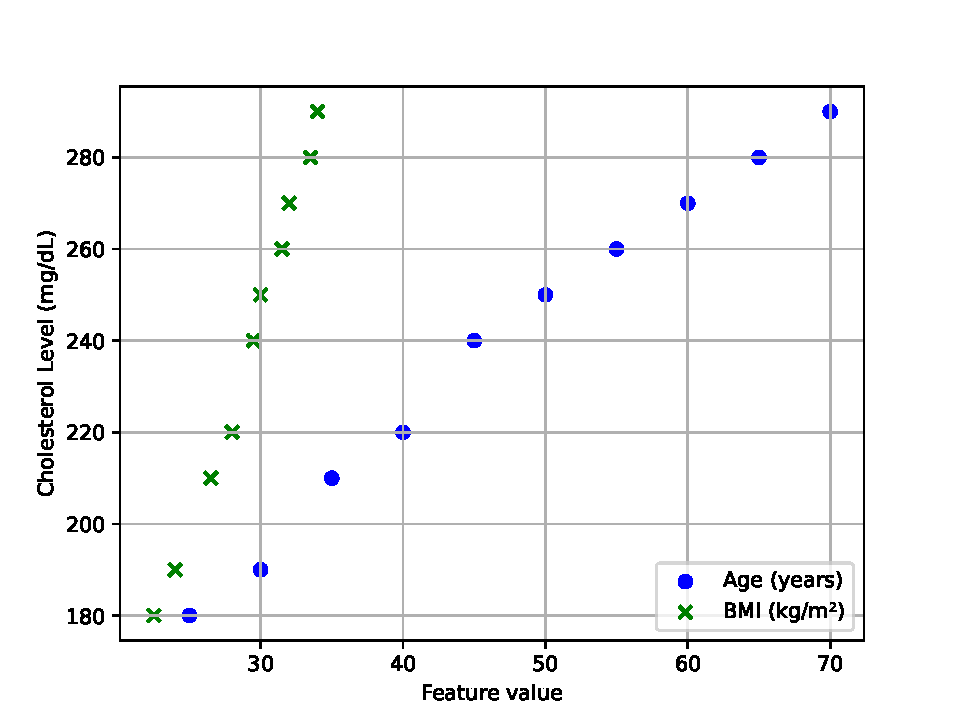
\includegraphics[width=0.49\columnwidth]{./figures/lin_reg_example/age_and_bmi_vs_cholesterol.pdf}
    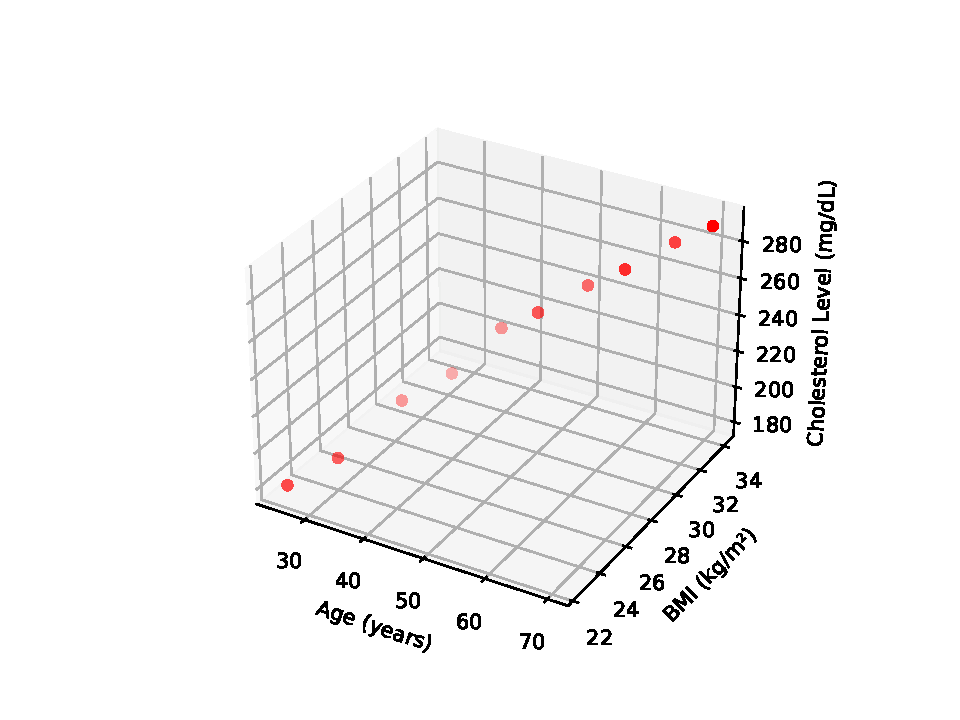
\includegraphics[width=0.49\columnwidth]{./figures/lin_reg_example/age_vs_bmi_vs_cholesterol.pdf}
    \caption{\centering Each feature against the output (left) and the dataset in the feature space (right).}
    \label{fig:not_at_all_the_same}
\end{figure}

\noindent Looks sufficiently linear to me. We'll split the dataset into training and testing datasets via \autoref{tab:lin_reg_example_train} and \autoref{tab:lin_reg_example_test}.
\begin{table}[ht]
    \begin{center}
        \begin{minipage}{0.49\textwidth}
            \begin{center}
                \begin{tabular}{c|c||c}
                    Age & BMI & Cholesterol\\
                    \hline
                    \hline
                    25 & 22.5 & 180 \\
                    35 & 26.5 & 210 \\
                    45 & 29.5 & 240 \\
                    55 & 31.5 & 260 \\
                    65 & 33.5 & 280 \\
                    \hline
                \end{tabular}
                \caption{\centering Training dataset.}
                \label{tab:lin_reg_example_train}
            \end{center}
        \end{minipage} \hfill
        \begin{minipage}{0.49\textwidth}
            \begin{center}
                \begin{tabular}{c|c||c}
                    Age & BMI & Cholesterol\\
                    \hline
                    \hline
                    30 & 24.0 & 190 \\
                    40 & 28.0 & 220 \\
                    50 & 30.0 & 250 \\
                    60 & 32.0 & 270 \\
                    70 & 34.0 & 290 \\
                    \hline
                \end{tabular}
                \caption{\centering Testing dataset.}
                \label{tab:lin_reg_example_test}
            \end{center}
        \end{minipage}
    \end{center}
\end{table}
Since $\Dtrain$ consists of only five samples, it's feasible to write out the optimal parameters $\thetaOpt$ by hand. We have
$$
y=
\begin{bmatrix}
    180\\
    210\\
    240\\
    260\\
    280\\
\end{bmatrix},
\hspace{10pt}
X=
\begin{bmatrix}
    1 & 25 & 22.5 \\
    1 & 35 & 26.5 \\
    1 & 45 & 29.5 \\
    1 & 55 & 31.5 \\
    1 & 65 & 33.5
\end{bmatrix}
$$
from which we obtain
$$
\thetaOpt
=
\left(X^{\T}X\right)^{-1}X^{\T}y
=
\begin{bmatrix}
    25.68\\
    0.94\\
    5.79
\end{bmatrix}
$$
which corresponds to
$$
f(x_1,x_2)=25.68+0.94x_1+5.79x_2.
$$

What's nice about such a low-dimensional problem like this is that visualising the loss landscape is relatively doable. We have three parameters so I'll fix $\theta_0=25.68$ and plot $\theta_1$ and $\theta$ against 
$$
\text{MSE}(25.68, \theta_1, \theta_2)
=
\sum_{i=1}^5 (y_i-25.68-\theta_1\x_{1,1}-\theta_2\x_{1,2})^2
$$
where the sum is taken over the training data $\{(\x_i,y_i)\}_{i=1,\dots,5}$.

As for how well the model performs, its MSE on $\Dtrain$ is $1.26$ and its MSE on $\Dtest$ is $12.24$. In this case, such a difference is fine. To get a visual on how well the model does on the training and testing sets, consider \autoref{lin_reg_example_on_train_and_test}. I should improve these at some point.

\begin{figure}[ht]
    \centering
    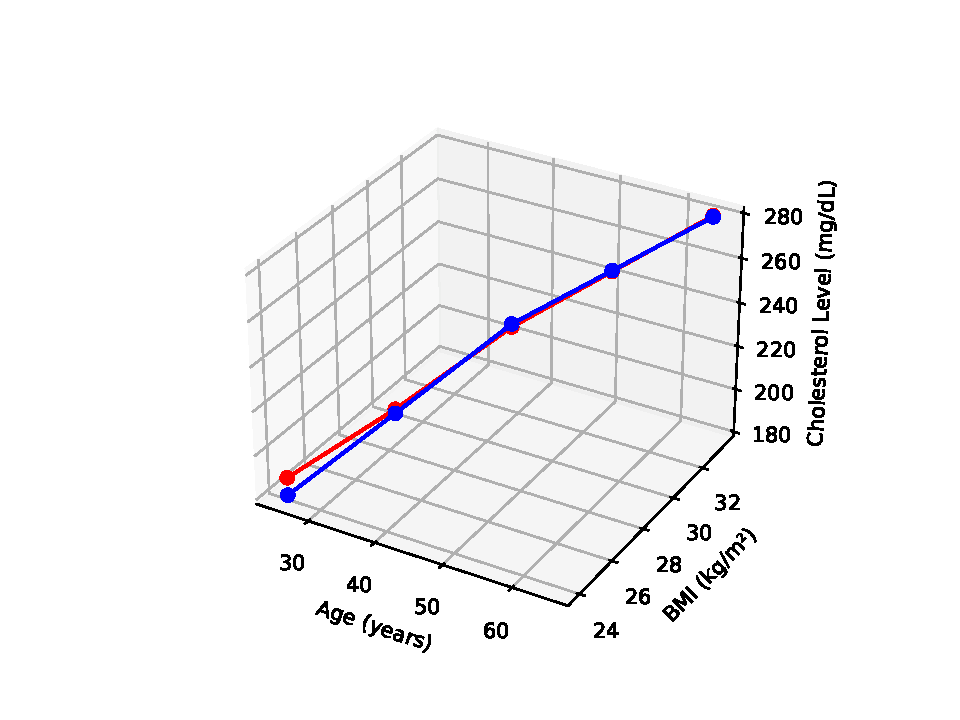
\includegraphics[width=0.49\columnwidth]{./figures/lin_reg_example/model_predicts_train.pdf}
    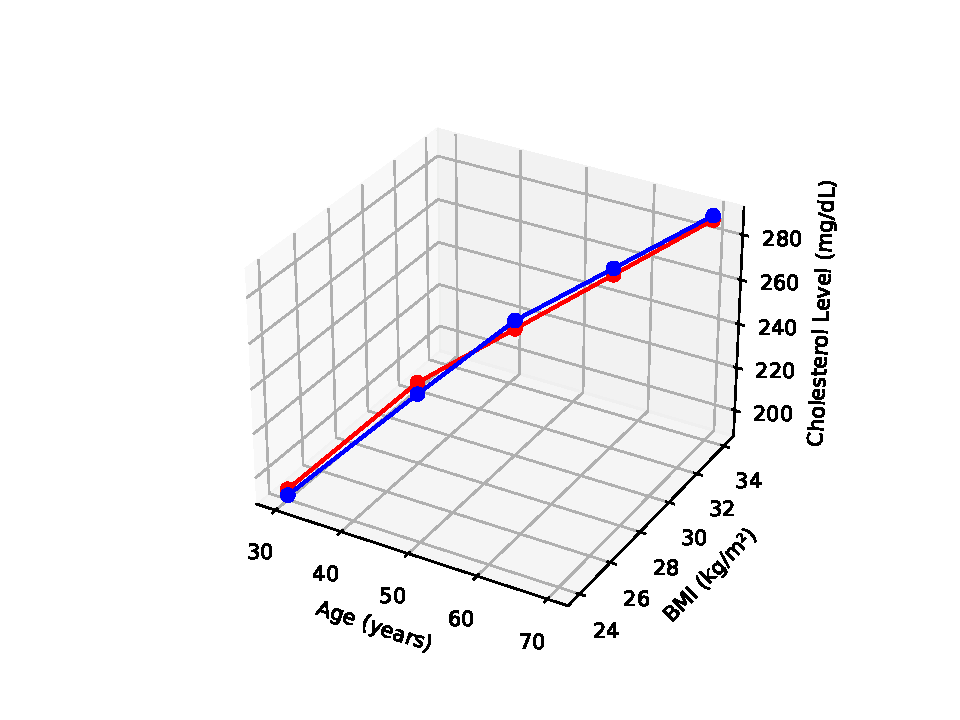
\includegraphics[width=0.49\columnwidth]{./figures/lin_reg_example/model_predicts_test.pdf}
    \caption{\centering Model performance on the training set (left) and testing set (right).}
    \label{fig:lin_reg_example_on_train_and_test}
\end{figure}

\begin{tcolorbox}[colback=c2]
    \textbf{Funny misuse of linear regression - Momentous sprint at the 2156 Olympics?}
    \vspace{10pt}

    The following is taken from an answer on Quora\footnote{\url{https://qr.ae/pslbEN}} (the top comment is worth reading) based on a paper\footnote{\url{https://www.ncbi.nlm.nih.gov/pmc/articles/PMC3173856/}} published in Nature. Related\footnote{\url{https://xkcd.com/1007/}}.
\end{tcolorbox}

\subsubsection{Regularisation}
Ridge regression intentionally introduces bias with the intention of reducing variance and improve accuracy!

\subsubsection{$R^2$ value}
\dots

\begin{tcolorbox}[colback=c2]
    \textbf{Assumption of normally distributed residuals}
    \vspace{10pt}

    Central limit theorem to the rescue!\footnote{\url{https://en.wikipedia.org/wiki/Central\_limit\_theorem\#Regression}} ``Regression analysis, and in particular ordinary least squares, specifies that a dependent variable depends according to some function upon one or more independent variables, with an additive error term. Various types of statistical inference on the regression assume that the error term is normally distributed. This assumption can be justified by assuming that the error term is actually the sum of many independent error terms; even if the individual error terms are not normally distributed, by the central limit theorem their sum can be well approximated by a normal distribution."
\end{tcolorbox}

\subsubsection{Terminology}

Nowadays, regression models are those which predict a value belonging to some continuous space but where did it come from? In 1886, Francis Galton authored ``Regression Towards Mediocrity in Hereditary Stature'' which is where the `regression towards the mean' term comes from. Galton noticed that tall father's have short sons, short fathers have tall sons and average height fathers have average height sons. Taken from a Stack Exchange comment: ``Galton derived a linear approximation to estimate a son's height from the father's height in that paper. His equation was fitted so an average height father would have an average height son, but a taller than average father would have a son that is taller than average by 2/3 the amount his father is. Same with shorter than average. This could be argued to be a simple linear regression."

Put mathematically, suppose random variables $X$ and $Y$ are related via $Y=\alpha+\beta Y+\epsilon$ where $\alpha,\beta\in\R$ are regression coefficients and $\epsilon$ is noise with mean $0$. Then $\E[Y|X]=\alpha+\beta X$, so if we first normalise to have RVs of mean 0 and variance 1 then we would have $E[Y|X]=\rho X$ where $\rho$ is the correlation coefficient between $X$ and $Y$. Since $|\rho|\leq1$ we know that the expected value of $Y$ is close to the mean than $X$ unless $\rho=1$. So extreme values of $X$ tend to correspond to values of $Y$ that are closer to the mean, i.e. one has regression towards the mean.

To see why this does not apply to all modern `regression' models, consider logistic regression in which one, roughly speaking, predicts probabilities of binary outcomes. In such cases, the dependent variable is binary, so `regressing towards the mean' has no meaningful interpretation.

The `linear' part refers to the output variable being linear in the parameters. This is sometimes confusing in linear regression we typically deal with basis functions that give line-like surfaces (lines, planes, etc.) but we could always have non-linear basis functions. For example, $y=\beta_0+\beta_1 e^x$ is linear in $\beta=(\beta_0,\beta_1)$ but $y=\beta_0+e^{\beta_1}x$ is not. A consequence is that an estimate $\hat{\beta}$ of the model parameters can be written as $\hat{\beta}=\sum_{i=1}^k w_iy_i$ where $w_i$ are the determined weights and $y_i$ are the chosen basis functions.

% how good is good data
\subsubsection{Opportunity to Demonstrate High Quality Data}

Let's say we had perfect data. That is, no noise and samples truly lie on the underlying hyperplane fit. In such a case, if our samples are of the form $(x_1,\dots,x_n,y)\in\R^{n+1}$ then the hyperplanes of interest are $n$-dimensional (assuming independent features?) and each is uniuely identified by $n+1$ distinct points on the plane. So if our data is perfect then bam, all we need is $n+1$ linearly independent samples to perfectly fit the data in the linear regression case.

The idea of course extends to things like polynomial regression, just more points are needed depending on the degree.

% logistic regression
\subsection{Logistic Regression}

While linear regression is the staple example of regression models, its equivalent for binary classification is logistic regression. The name is a bit confusing at first since it's fair to expect that something with the name regression would be used for regression tasks, i.e. predicting something continuously distributed, as opposed to something discrete like binary classification. Logistic Regression essentially applies a logistic (or sigmoid) transformation to the output of our model to introduce a notion of confidence of the classification. Understandably, this transformation maps all outputs to $(0,1)$. This is what makes it regression-like.

Binary classification is the task of assigning one of two classes to some input sample. For example, given some data pertaining to a patient's health, it might be nice to be able to predict whether they are at risk of suffering from a heart attack or not. With this in mind, how does one classify a sample at all? The idea is to fit a hyperplane to the feature space of the distribution which we wish to model. A hyperplane is an $(n-1)$-dimensional object embedded in $n$-dimensional space. So in 2D space, a hyperplane is just a line and in 3D space it's a plane etc. A hyperplane in $(p+1)-$dimensional space consists of the points $(x_1,\dots,x_p)\in\R^p$ which satisfy
$$
\theta_0+\theta_1x_1+\dots+\theta_px_p=0
$$
where $\theta=(\theta_0,\dots,\theta_p)$ are the hyperplane's coefficients and $\x=(1,x_1,\dots,x_p)$ and we can denote the function corresponding to the hyperplane by
$$
f_{\theta}(\x)
=
\theta_0+\theta_1x_1+\dots+\theta_px_p
=
\theta^{\text{T}}\x.
$$
The reason for the additional $1$ appearing at the beginning of $\x$ is similar to as in linear regression: it accounts for the bias term $\theta_0$ and makes notation a lot cleaner. After fitting the parameters of such a hyperplane, we can classify a sample $\x$ according to which side of the hyperplane $f_{\theta}(\x)=0$ it lies. For example, samples `below' the hyperplane, i.e. $f_{\theta}(\x)\leq0$, are classified as $0$ and samples `above', i.e. $f_{\theta}(\x)>0$, are classified as $1$. With this idea in mind, the hard part of this approach is finding an appropriate hyperplane. That is, we want $f_{\theta}(\x)$ to be such that sufficiently many samples of each class lie on the correct side of the hyperplane. To regressionify this approach, we apply a logistic transformation to the output $f_{\theta}(\x)$ for a given sample $\x$ yielding
$$
h_{\theta}(\x)
=
\sigma(f_{\theta}(\x))
=
\frac{1}{1+\exp(-f_{\theta}(\x))}\in(0,1)
$$
and say that sample $\x$ is of class $1$ if $h_{\theta}(\x)>p$, for some pre-determined threshold $p\in(0,1)$, and of class $0$ if $h_{\theta}(\x)\leq p$. So ultimately, $C_{\theta}(\x)=I(h_{\theta}(\x)>p)$ where $I$ denotes the indicator function. Typically, people take $p=0.5$ which yields precisely the same classifications as $f_{\theta}(\x)$. To see this, note that if $p=0.5$ then we have
\begin{align*}
    C_{\theta}(\x)=1
    \iff & h_{\theta}(\x)>0.5\\
    \iff & \frac{1}{1+\exp(-f_{\theta}(\x))}>0.5\\
    \iff & 1 > \exp(-f_{\theta}(\x))\\
    \iff & f_{\theta}(\x) > 0\\
    \iff & \theta^{\T}\x > 0.
\end{align*}

\noindent Like in linear regression, for a statistical motivation we'll make some assumptions regarding the class labels to derive a way of finding the optimal parameters $\thetaOpt$.

\subsubsection{Statistical Motivation}
Suppose that the outputs of the logistic function $h_{\theta}$ are Bernoulli distributed with parameter $p$. That is, suppose that $h_{\theta}(\x)\sim\text{Bernoulli}(p)$. In this case, the probability that $\x$ belongs to class $y\in\{0, 1\}$ is given by
$$
\P(y|\x;\theta)=(h_{\theta}(\x))^{y}(1-h_{\theta}(\x))^{1-y}.
$$
We construct the log-likelihood of $h_{\theta}(\x)$ over $\Dtrain=\{(\x_i,y_i)\}_{i=1}^n$, assuming its samples are i.i.d., as
\begin{align*}
    l(\theta)
    &=
    \sum_{i=1}^n\log(\P(y_i|\x_i;\theta))\\
    &=
    \sum_{i=1}^n\log\left((h_{\theta}(\x_i))^{y_i}(1-h_{\theta}(\x_i))^{1-y_i}\right)\\
    &=
    \sum_{i=1}^ny\log(h_{\theta}(\x_i))+(1-y_i)\log(1-h_{\theta}(\x_i))\\
    &=
    \sum_{i=1}^n\left[y_i\log\left(\frac{1}{1+\exp(-\theta^{\T}\x_i)}\right)+(1-y_i)\log\left(1-\frac{1}{1+\exp(-\theta^{\T}\x_i)}\right)\right]\\
    &=
    \sum_{i=1}^n\left[y_i\log\left(\frac{1}{1+\exp(-\theta^{\T}\x_i)}\right)+(1-y_i)\log\left(\frac{\exp(-\theta^{\T}\x_i)}{1+\exp(-\theta^{\T}\x_i)}\right)\right]\\
    &=
    \sum_{i=1}^n\left[y_i\log\left(\frac{1}{1+\exp(-\theta^{\T}\x_i)}\right)+(1-y_i)\left(-\theta^{\T}\x_i+\log\left(\frac{1}{1+\exp(-\theta^{\T}\x_i)}\right)\right)\right]\\
    &=
    \sum_{i=1}^n\left[-\log(1+\exp(-\theta^{\T}\x_i))-(1-y_i)\theta^{\T}\x_i\right]
\end{align*}
which we maximise using something like gradient descent to obtain the optimal paramateres
$$
\thetaOpt
=
\argmax_{\theta\in\R^{p+1}}\left[\sum_{i=1}^n\left[-\log(1+\exp(-\theta^{\T}\x_i))-(1-y_i)\theta^{\T}\x_i\right]\right].
$$

\noindent\textbf{Note:} In practice, it's unlikely that any samples will lie on the hyperplane $f_{\theta^*}(\x)=0$ itself.

% support vector machines
\subsection{Support Vector Machines (SVMs)}
Logistic regression and SVMs both fit a hyperplane in feature space. The distinction is the metric of goodness of said hyperplanes. In logistic regression, the metric of goodness is how much the parameters of said hyperplane maximise the relevant log-likelihood. SVMs, however, look to maximise the distance between the hyperplane and the samples. So in some sense, logistic regression is a probabilistic approach while SVMs take more of a classic approach of `maximise this thing according to well-defined contraints'.

The authors' insight came from structural risk minimization in which instead of focusing on minimising training error (as neural networks and decision trees were doing at the time), one focuses on minimising an upper bound on the generalisation error. The inclusion of `support vector' is clear from their construction but `machine' stood out to me as a bit odd. It turns out that at time of their development, around 1960, it was common to use `machine' when referring to algorithms that learned from data, i.e. algorithms belonging to statistical learning theory.\\

\noindent\textbf{Note:} Terminology surrounding SVMs is inconsistent. Some pieces of literature describe the decision boundary learned by an SVM as strictly linear, others allow for a non-linear decision boundary. It'd be nice if authors stuck to the former and explicitly stated `non-linear SVM' when describing the latter. Here, `an SVM' refers to the former and I'll state explicitly when considering the latter.

\subsubsection{Hard-margin SVMs}
Since we aim to fit a hyperplane in our feature space $\R^{p+1}$, we use the same notation for the function $f_{\theta}(\x)$ corresponding to the linear decision boundary (i.e. hyperplane). To make notation a bit easier, let $\theta_+=(\theta_1,\dots,\theta_p)$ so that $\theta$ is the ordered concatentation of $\theta_0$ and $\theta_+$. Further, let $\x_i$ denote the $i^{\text{th}}$ sample's features and $z_i\in\{-1,1\}$ its class such that $z_i$ is 1 if $\theta_+^{\text{T}}\x_i+\theta_0>0$ and 0 otherwise.

\begin{figure}[ht]
    \centering
    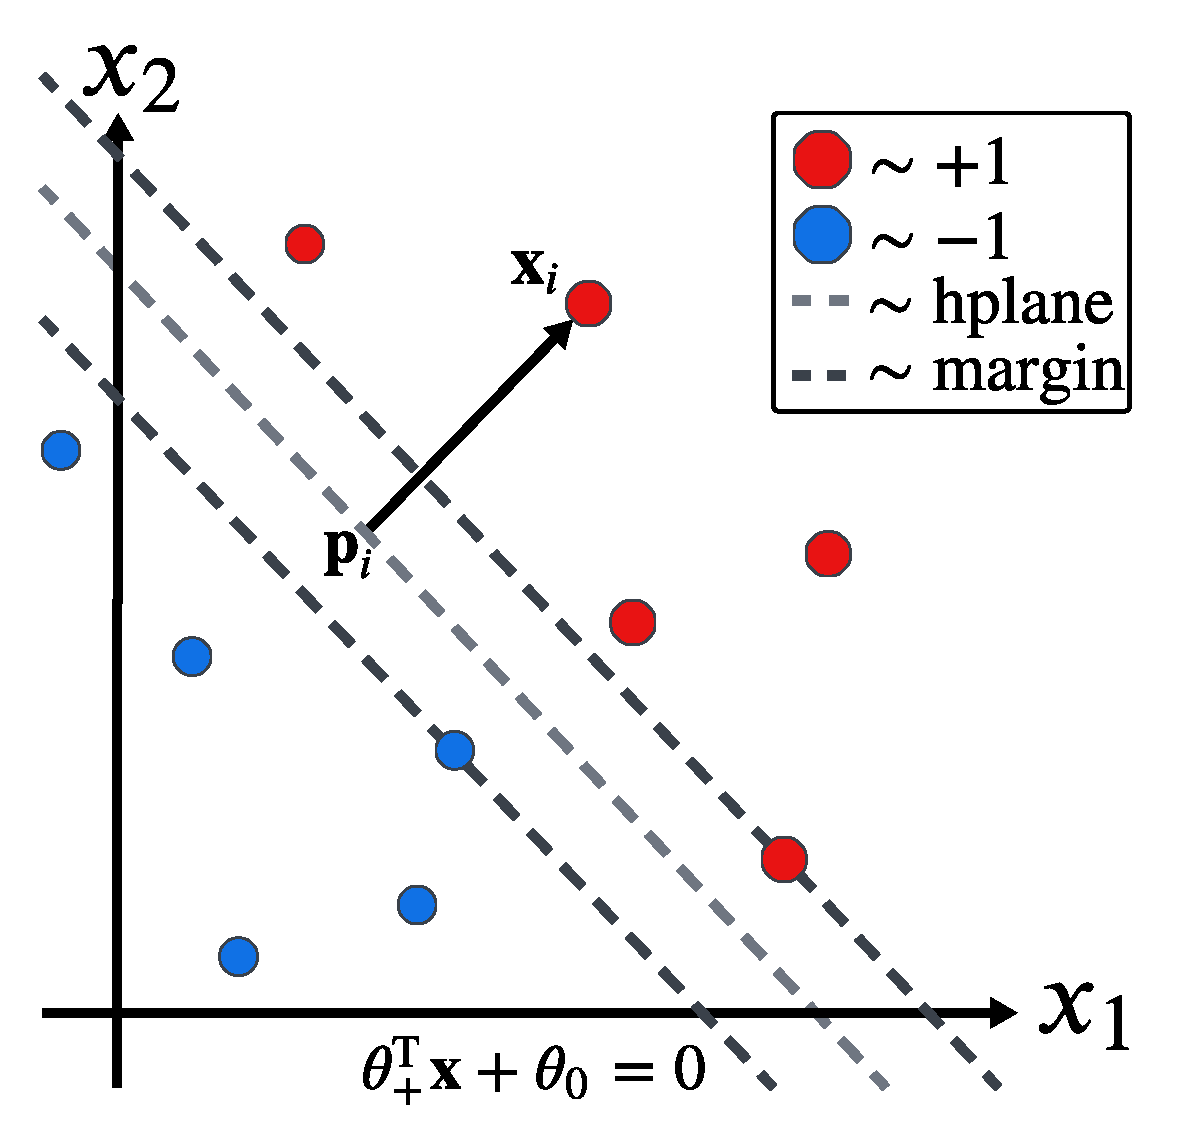
\includegraphics[width=0.5\columnwidth]{./figures/SVMs/SVM_hard_margin.pdf}
    \caption{\centering A hard-margin SVM in two dimensions.}
    \label{fig:SVM_hard_margin}
\end{figure}

\noindent Let $\mathbf{p}_i$ denote the projection of $\x_i$ onto the hyperplane and let $d_i$ denote the distance between $\mathbf{p}_i$ and $\x_i$. Noting that the normal to the hyperplane is $\theta_+$, we have $\mathbf{p}_i=\x_i-\frac{\theta_+}{||\theta_+||}d_i$ and so
$$
\theta_+^{\text{T}}\left(\x_i-\frac{\theta_+}{||\theta_+||}d_i\right)+\theta_0
=
0
$$
which, after some rearranging, yields
$$
d_i
=
\frac{\theta_+^{\text{T}}\x_i+\theta_0}{||\theta_+||}.
$$
Taking a point $\x_i$ whose class is $-1$ yields $d_i=-\frac{\theta_+^{\text{T}}\x_i+\theta_0}{||\theta_+||}$ and so a neater way of writing this distance for an arbitrary sample $\x_i$ is $d_i=\frac{z_i(\theta_+^{\text{T}}\x_i+\theta_0)}{||\theta_+||}$. Let $d_{\text{min}}=\min_{i=1,\dots,n}d_i$. The idea behind hard-margin SVMs is only applicable to entirely linearly sparable data and effectively boilds down to finding which parameters maximise $d_{\text{min}}$. That is, we look to compute
\begin{align*}
    \thetaOpt
    &=
    \argmax_{(\theta_0,\theta_+)}\left[\min_{i=1,\dots,n}d_i\right]\\
    &=
    \argmax_{(\theta_0,\theta_+)}\left[\min_{i=1,\dots,n}\frac{z_i(\theta_+^{\text{T}}\x_i+\theta_0)}{||\theta_+||}\right]\\
\end{align*}
which we'd like to translate into a convex optimisation problem. First, notice that computing $\thetaOpt$ is equivalent to solving
$$
\max_{(\theta_0,\theta_+)}\frac{r}{||\theta_+||}\text{ s.t. } z_i\left(\theta_+^{\text{T}}\x_i+\theta_0\right)\geq r\text{ } (i=1,\dots,n).
$$
in which $r$ is arbtirarily scalable, so it is equivalent to
$$
\max_{(\theta_0,\theta_+)}\frac{1}{||\theta_+||}\text{ s.t. } z_i\left(\theta_+^{\text{T}}\x_i+\theta_0\right)\geq 1\text{ } (i=1,\dots,n).
$$
This problem is still non-convex so we make a convenient switcheroo in realising that it is equivalent to solving
$$
\min_{(\theta_0,\theta_+)}||\theta_+||^2\text{ s.t. } z_i\left(\theta_+^{\text{T}}\x_i+\theta_0\right)\geq 1\text{ } (i=1,\dots,n)
$$
which is solved in the usual convex problem solving ways.

\subsubsection{Soft-margin SVMs}

Hard-margin SVMs are rarely applicable. In practice, classes are not entirely linearly separable, due to noise and outliers, and so allowing for some misclassification is pragmatic. Going from hard-margin to soft-margin is pretty straightforward, just include some slack variables $\xi=(\xi_1,\dots,\xi_n)$ that ultimately allow the model to violate the constraints while penalising said violations. More precisely, it involves solving
$$
\min_{(\theta_0,\theta_+,\xi)}\left[||\theta_+||^2+\lambda\sum_{i=1}^n\xi_i\right]\text{s.t. } z_i\left(\theta_+^{\text{T}}\x_i+\theta_0\right)\geq 1-\xi_i,\text{ }\xi_i\geq0\text{ } (i=1,\dots,n)
$$
where $\lambda\geq0$ is a regularisation parameter that influences the tradeoff of margin size and misclassification rate. Larger $\lambda$ corresponds to prioritising a larger margin while smaller $\lambda$ corresponds to prioritising the minimisation of misclassification.

\begin{figure}[ht]
    \centering
    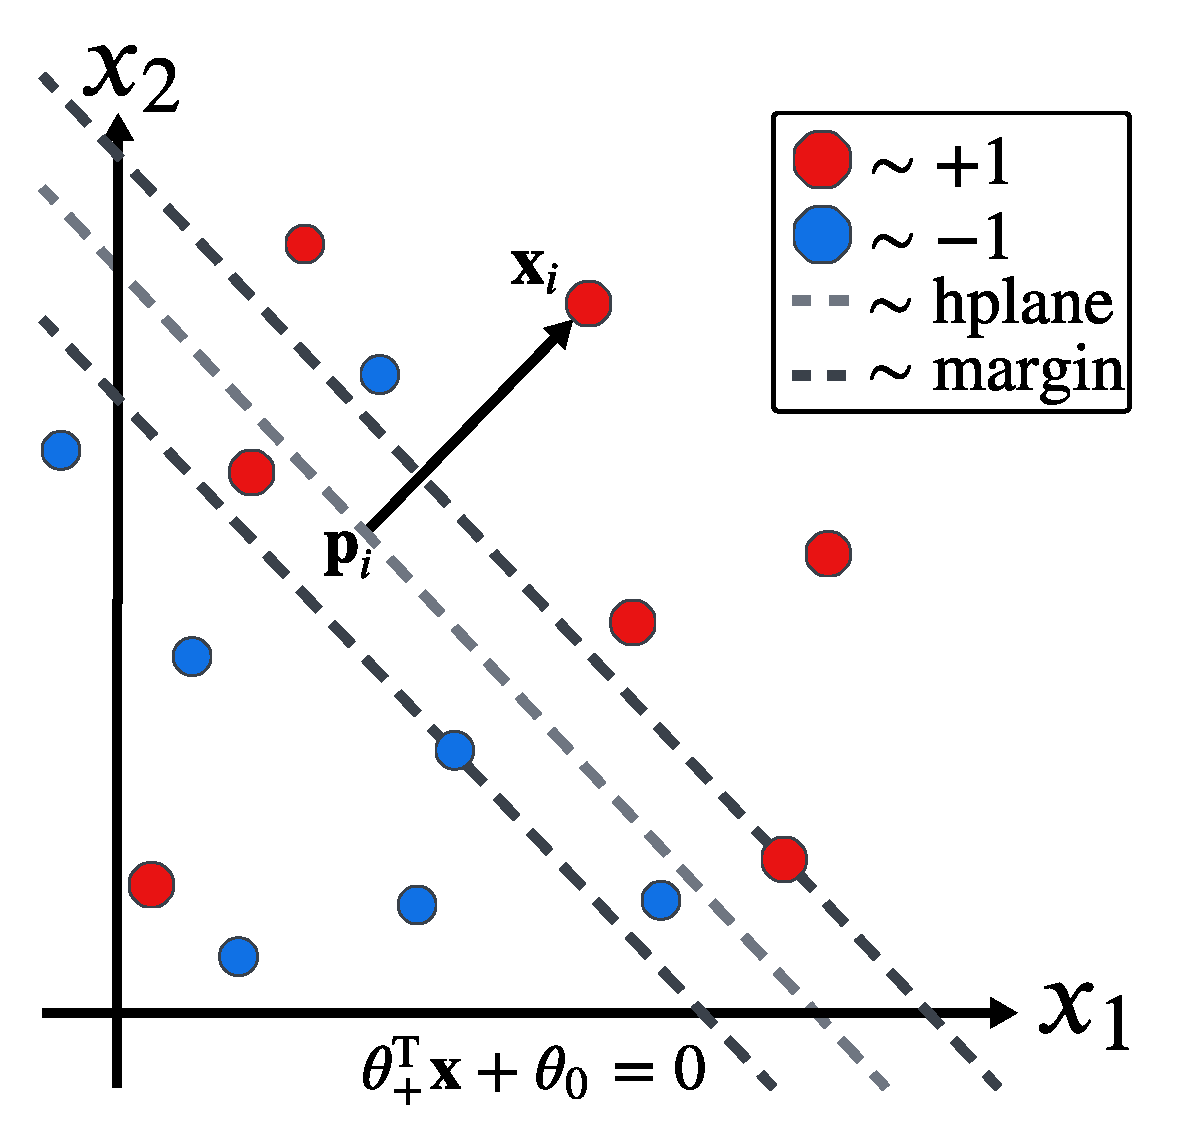
\includegraphics[width=0.5\columnwidth]{./figures/SVMs/SVM_soft_margin.pdf}
    \caption{\centering A soft-margin SVM in two dimensions. Samples are labelled according to their true class.}
    \label{fig:SVM_soft_margin}
\end{figure}

\noindent As illustrated in \autoref{fig:SVM_soft_margin}, it allows for samples to be closer to the decision boundary than the margin as well as outright misclassifications. Again, it is typically solved in the usual convex problem solving ways. Going a step further, it turns out that this can be simplified to computing
$$
\argmin_{(\theta_0,\theta_+)}\left[||\theta_+||^2+\lambda\sum_{i=1}^n\max\left(0,1-z_i\left(\theta_+^{\text{T}}\x_i+\theta_0\right)\right)\right]
$$
which can be done using gradient descent.

\subsubsection{Non-linear SVMs}
\begin{itemize}
    \item the kernel trick
    \item standard kernels
    \item derivation of standard identity
\end{itemize}
\dots

% decision trees and random forests
\subsection{Decision Trees and Random Forests}
\begin{itemize}
    \item split according to some feature
    \item i love democracy, prune them
\end{itemize}

% handcrafted features
\subsection{Handcrafted Features}
\dots

% the bias-variance tradeoff
\subsection{The Bias-Variance Trade-Off}
\dots

\subsubsection{Double descent}
\dots

% misc. questions
\addtocontents{toc}{\protect\setcounter{tocdepth}{1}}
\subsection{Misc. questions}
\addtocontents{toc}{\protect\setcounter{tocdepth}{2}}

Some questions to challenge one's understanding.

\begin{tcolorbox}[colback=c2]
\begin{center}
    \textbf{Q1: What are the benefits of using logistic regression over more sophisticated methods?}
\end{center}
\vspace{-8pt}
\begin{itemize}
    \item Its implementation and interpretation are straightforward
    \item If offers a notion of classification confidence which can be useful
    \item Statistical tests can be conducted on parameters, e.g. statistical significance tests
    \item mention more classical statistics approaches like LDA and QDA
\end{itemize}
\end{tcolorbox}

\begin{tcolorbox}[colback=c2]
\begin{center}
    \textbf{Q2: Why not use mean absolute error instead of MSE?}
\end{center}
\vspace{-8pt}
There are many reasons for this, one of which is that often in machine learning and statistics-related contexts one would like to be able to compute the derivative(s) of such a loss function, e.g. in gradient descent, and the presence of an absolute value makes this annoying.

As to why it's useful that the MSE involves the squares of the errors, instead of exponents like $2.05, 3$ or $\pi$, it was best put by this answer to a Stack Exchange answer about the same question\footnote{\url{https://math.stackexchange.com/a/63245}}:

``The variance is the mean squared deviation from the average. The variance of the sum of 10,000 random variables is the sum of their variances. That doesn't work for other powers of the absolute value of the deviation. That means if you roll a die 6,000 times, so that the expected number of 1s you get is 1,000, then you also know that the variance of 1s is $6000\cdot\frac{1}{6}\cdot\frac{5}{6}$ so if you want the probability that the numbner of 1s is between 990 and 1,020, you can approximate the distribution by the normal distribution with the same mean and variance. You couldn't do that if you didn't know the variance, and you couldn't know the variances without additivity of variances, and if the exponent were anything besides 2, then you don't have that. (Oddly, you do have additivity with cubes of the deviations, but not cubes of the absolute values of the deviations)."
\end{tcolorbox}

\begin{tcolorbox}[colback=c2]
\begin{center}
    \textbf{Q3: How can we get an idea of the extent to which our features and output are linearly related without plotting?}
\end{center}
\vspace{-8pt}
To be honest, I thought a streamline test for this existed. As per this Stack Exchange answer\footnote{\url{https://stats.stackexchange.com/a/239142}}, a good method for this is to simply fit a linear and a non-linear model (e.g. a cubic spline smoother model) and see which explains a larger amount of the variance of the output via ANOVA tests.
\end{tcolorbox}

% gradient descent and optimisation techniques
\section{Gradient Descent and its Optimisation}
\dots

% vanilla gradient descent
\subsection{Gradient Descent}
How do we find such an appropriate set of weights and biases for a neural network? More generally, how do we find an appropriate set of parameters for a machine learning model? A popular method is that of gradient descent.

% momentum
\subsection{Momentum}
\dots

% hyperparam tuning
\subsection{Hyperparameter Tuning}
cross-validation and shiiiiiiieeet

% misc. questions
\addtocontents{toc}{\protect\setcounter{tocdepth}{1}}
\subsection{Misc. questions}
\addtocontents{toc}{\protect\setcounter{tocdepth}{2}}

Some questions to challenge one's understanding.

\begin{center}
    \textbf{\textcolor{blue}{Q1:} ?}
\end{center}
\dots

\subsubsection{Why does $f(\mathbf{x})$ ascend most in the direction of $\nabla f(\mathbf{x})$?}

The following is more of a proof \textit{that} $\nabla f(x)$ yields the direction of steepest ascent not an intuition of \textit{why}. That'll come later.

For some reason, it is typically taken for granted that $f(\mathbf{x})$ would both ascend and ascend \textit{most} in the direction of $\nabla f(\mathbf{x})$. I do not consider this obvious at all, so here is an informal physicist-like argument. Note that in this argument, we consider only unit vectors $\mathbf{v}$. This is because we care only about the direction of such vectors, so size does not matter, and an equation later on simplifies quite nicely due to its unit length. 

In gradient descent, we are looking for the unit vector $\mathbf{v}$ such that $f(\mathbf{x})$ increases most in the direction of $\mathbf{v}$, i.e. we are trying to solve the optimisation problem given by
$$\argmax_{||\mathbf{v}||=1}\Big[f(\mathbf{x}+\eta\mathbf{v})-f(\mathbf{x})\Big]$$
where $\eta>0$. Approximating $f(\mathbf{x}+\eta\mathbf{v})$ by its Taylor approximation
$$
\nabla f(\mathbf{x})\cdot\mathbf{v}\approx\frac{f(\mathbf{x}+\eta\mathbf{v})-f(\mathbf{x})}{\eta},
$$
for small $\eta>0$, yields
$$
f(\mathbf{x}+\eta\mathbf{v})-f(\mathbf{x})
\approx
\nabla f(\mathbf{x})\cdot\eta\mathbf{v}
$$
and so the problem translates to finding the unit vector $\mathbf{v}$ that maximises
$$
\nabla f(\mathbf{x})\cdot\eta\mathbf{v}=||\nabla f(\mathbf{x})||\cdot||\eta\mathbf{v}||\cdot\cos(\theta)=\eta||\nabla f(\mathbf{x})||\cdot\cos(\theta)
$$
where $\theta\in[0,\pi)$ denotes the angle between $\nabla f(\mathbf{x})$ and $\mathbf{v}$. This is clearly maximised when $\cos(\theta)=1$, i.e. when $\theta=0$, and $\mathbf{v}$ has the same direction as $\nabla f(\mathbf{x})$. So $\mathbf{v}$ is a unit vector in the direction of $\nabla f(\mathbf{x})$, i.e. $\mathbf{v}=\frac{\nabla f(\mathbf{x})}{||\nabla f(\mathbf{x})||}$. To see that $f$ ascends after being sent in the direction of $\mathbf{v}=\frac{\nabla f(\mathbf{x})}{||\nabla f(\mathbf{x})||}$ from $\mathbf{x}$ by a distance $\eta>0$, note that
$$
f(\mathbf{x}+\eta\mathbf{v})-f(\mathbf{x})
\approx
\nabla f(\mathbf{x})\cdot\eta\mathbf{v}
=
\eta\frac{\nabla f(\mathbf{x})\cdot\nabla f(\mathbf{x})}{||\nabla f(\mathbf{x})||}
=
\eta||\nabla f(\mathbf{x})||
>
0.
$$
The edge case where $\nabla f(\mathbf{x})=0$ of course corresponds to $f(\mathbf{x})$ being a local maximum.

\vspace{10pt}

\noindent\textbf{Note}: This argument, which utilises a Taylor approximation, relies on a sufficiently small $\eta>0$. Otherwise, the terms in the Taylor approximation of $f(\mathbf{x}+\eta\mathbf{v})$ beyond $\nabla f(\mathbf{x})\cdot\eta\mathbf{v}$ are not necessarily negligible.

\subsubsection{Choosing a loss function}
Note that these depend on having uniform diversity of classes. If not then use weighted cross-entropy loss functions. There are a ton of machine learning-related scenarios that would need a specially chosen loss function but the list below is a fine start. 123

\begin{table}[ht]
    \begin{center}
        \begin{tabular}{c||c}
            \textbf{Task} & \textbf{Loss function}\\
            \hline
            \hline
            Binary classification & Binary cross-entropy\\
            Multi-class classification & Categorical cross-entropy\\
            Regression & Mean square error\\
            Multi-label classification & Binary cross-entropy over each label\\
            \hline
        \end{tabular}
    \end{center}
    \vspace{-15pt}
    \caption{\centering Loss function choices.}
    \label{tab:loss_func_choices}
\end{table}

\subsubsection{How should we choose the learning rate $\eta$?}
This is entirely problem-dependent but $\eta=0.1$ is a great staple choice. If convergence is unstable then try $\eta=0.01$. Other than this line of thinking, there are some `rules of thumb' relating batch number/size to learning rate, otherwise it's a `whatever seems to work best' kind of thing.

\subsubsection{How should we initialise the parameters?}
\dots

% deep learning
\newpage
\section{Neural Networks}
It is often the case that what people mean when they state `neural networks' they more precisely mean multi-layer perceptrons (MLPs), perhaps the simplest kind of neural network. Rigorously formulating MLPs is one of those things that's useful to do at least once. Formulating more sophisticated architectures, like CNNs, RNNs, etc., can be done in a much less rigorous manner when all we really want to do with them is solve tasks in an engineery way.

% neural networks
\subsection{Multi-Layer Perceptrons (MLPs)}

Multi-layer perceptrons (MLPs)footnote{\url{https://stats.stackexchange.com/a/159172}} are fully-connected feed-forward networks consisting of an input layer (where data is input), hidden layers and an output layer. An MLP with three hidden layers is illustrated in \autoref{fig:MLP}. Each layer is made up of a number of neurons, each of which has a real-valued activation value.  For any node in a non-input layer, its activation value is the output of a non-linear activation function given, as input, the node's real-valued bias plus a weighted sum of the activation values of the neurons in its preceding layer.

The application of MLPs to learning functions from data is due to their expressivity and their expressive-efficiency. Their expressivity is known due to a proof of the universal function approximation of MLPs by Cybenko \cite{universal_approx_theorem}. To add to this, their high expressive-efficiency has been demonstrated empirically \cite{exp_eff_of_MLPs} and ensures that the number of model components (hidden layers and neurons) needed to represent arbitrary functions is often far lower than competing methods.

\begin{figure}[H]
    \centering
    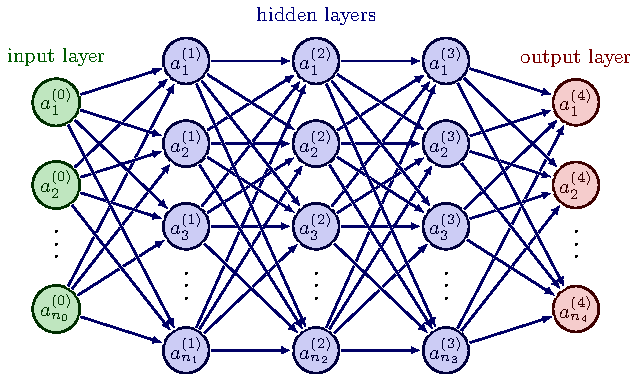
\includegraphics[width=1\linewidth]{./figures/neural_net_1.pdf}
    \caption{\centering A multi-layer perceptron (MLP) with $k=3$ hidden layers.}
    \label{fig:MLP}
\end{figure}
\noindent For ease of notation, given an MLP with $k$ hidden layers, denote the index of the input layer by $0$, the output layer by $k+1$ and by extension the $j^{\text{th}}$ layer by $j\in\{0,\dots,k+1\}$. Additionally, note the following:
\begin{itemize}
    \item Let $n_j\in\mathbb{Z}_{\geq1}$ denote the number of neurons in layer $j$.
    \item Let $a_i^{(j)}\in\mathbb{R}$ denote the activation value of neuron $i$ in layer $j$.
    \item Let $w_{i,l}^{(j)}\in\mathbb{R}$ denote the weight associated with the edge to neuron $i$ in layer $j\in\{1,\dots,k+1\}$ from neuron $l$ in layer $j-1$.
    \item Let $b_i^{(j)}\in\mathbb{R}$ denote the bias of neuron $i$ in layer $j\in\{1,\dots,k+1\}$.
    \item Let $\sigma_j:\mathbb{R}\rightarrow\mathbb{R}$ denote the non-linear activation function of layer $j\in\{1,\dots,k+1\}$.
\end{itemize}

\noindent From here we can express the activation value of any neuron in a non-input layer in terms of the activation values of the neurons in the layer which precedes it as
\begin{align*}
    a_i^{(j+1)}
    &=
    \sigma_{j+1}\left(
    \sum_{l=1}^{n_j} w_{i,l}^{(j+1)}a_l^{(j)} + b_i^{(j+1)}
    \right)\\
    &=
    \sigma_{j+1}\left(
    \left[w_{i,1}^{(j+1)} \dots w_{i,n_j}^{(j+1)}\right]
    \begin{bmatrix}
        a_1^{(j)}\\
        \vdots\\
        a_{n_j}^{(j)}
    \end{bmatrix}
    +
    b_i^{(j+1)}
\right)
\end{align*}
for $j\in\{0,\dots,k\}$. The reason for writing the second equality above, involving the dot product of two vectors, is that it helps us to see how using matrix-vector notation allows us to write an elegant and compact expression for the activation values of all nodes in a non-input layer in terms of the activation values of the neurons belonging to its preceding layer as
$$
\begin{bmatrix}
    a_1^{(j+1)}\\
    \vdots\\
    a_{n_{j+1}}^{(j+1)}
\end{bmatrix}
=
\sigma_{j+1}\left(
\begin{bmatrix}
    w_{1,1}^{(j+1)} & \dots & w_{1,n_j}^{(j+1)}\\
    \vdots & \ddots & \vdots\\
    w_{n_{j+1},1}^{(j+1)} & \dots & w_{n_{j+1},n_j}^{(j+1)}
\end{bmatrix}
\begin{bmatrix}
    a_1^{(j)}\\
    \vdots\\
    a_{n_j}^{(j)}
\end{bmatrix}
+
\begin{bmatrix}
    b_1^{(j+1)}\\
    \vdots\\
    b_{n_{j+1}}^{(j+1)}
\end{bmatrix}
\right)
$$
which we abbreviate to
$$
\mathbf{a}^{(j+1)}=\sigma_{j+1}\left(\mathbf{W}^{(j+1)}\mathbf{a}^{(j)}+\mathbf{b}^{(j+1)}\right)
$$
where the activation function $\sigma_{j+1}$ is applied element-wise.

If we fix the structure and choice of activation functions of an MLP then all that is left to learn are its weights and biases. This is often done using gradient descent to minimise some loss function in which gradients are computed via back-propagation \cite{backpropagation}. Such a loss function can be a principled measure, e.g. corresponding to maximum likelihood, but this is not always necessary: ad-hoc loss functions are sometimes employed.

\subsubsection{Constructive example - The algebra}

\begin{figure}[ht]
    \centering
    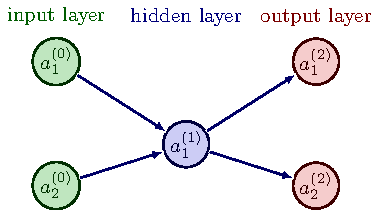
\includegraphics{./figures/neural_nets/neural_net_3.pdf}
    \caption{\centering A neural network with $k=1$ hidden layer.}
    \label{fig:neural_nets_simple_example}
\end{figure}

\noindent Consider the neural network in \autoref{fig:neural_nets_simple_example} whose input, hidden and output layers consist of two, one and two neurons respectively. With such a simple neural network, we may explicitly express the output neurons $a_1^{(2)}$ and $a_2^{(2)}$ in terms of the input neurons $a_1^{(0)}$ and $a_2^{(0)}$. We see that $n_0=2$, $n_1=1$ and $n_2=2$ and so
$\mathbf{W}^{(1)}=
\begin{bmatrix}
    w_{1,1}^{(1)} & w_{1,2}^{(1)}
\end{bmatrix}
$
and
$\mathbf{W}^{(2)}=
\begin{bmatrix}
    w_{1,1}^{(2)}\\
    w_{2,1}^{(2)}
\end{bmatrix}.
$
Noting additionally that $\mathbf{b}^{(1)}=b_1^{(1)}$ and
$\mathbf{b}^{(2)}=
\begin{bmatrix}
    b_{1}^{(2)}\\
    b_{2}^{(2)}
\end{bmatrix}$
we can explicitly express the activation of the single neuron in the hidden layer as
\begin{align*}
\mathbf{a}^{(1)}
&=
\sigma_1\left(\mathbf{W}^{(1)}\mathbf{a}^{(0)}+\mathbf{b}^{(1)}\right)\\
&=
\sigma_1\left(w_{1,1}^{(1)}a_1^{(0)}+w_{1,2}^{(1)}a_2^{(0)}+b_1^{(1)}\right)
\end{align*}
which is just the scalar value $a_1^{(1)}$. For the output layer, we have
\begin{align*}
\mathbf{a}^{(2)}
&=
\sigma_2\left(\mathbf{W}^{(2)}\mathbf{a}^{(1)}+\mathbf{b}^{(2)}\right)\\
&=
\sigma_2\left(
\begin{bmatrix}
    w_{1,1}^{(2)}a_1^{(1)} + b_1^{(2)}\\
    w_{2,1}^{(2)}a_1^{(1)} + b_2^{(2)}
\end{bmatrix}
\right)\\
&=
\sigma_2\left(
\begin{bmatrix}
    w_{1,1}^{(2)}\sigma_1\left(w_{1,1}^{(1)}a_1^{(0)}+w_{1,2}^{(1)}a_2^{(0)}+b_1^{(1)}\right) + b_1^{(2)}\\
    w_{2,1}^{(2)}\sigma_1\left(w_{1,1}^{(1)}a_1^{(0)}+w_{1,2}^{(1)}a_2^{(0)}+b_1^{(1)}\right) + b_2^{(2)}
\end{bmatrix}
\right)\\
&=
\begin{bmatrix}
    \sigma_2\left(w_{1,1}^{(2)}\sigma_1\left(w_{1,1}^{(1)}a_1^{(0)}+w_{1,2}^{(1)}a_2^{(0)}+b_1^{(1)}\right) + b_1^{(2)}\right)\\
    \sigma_2\left(w_{2,1}^{(2)}\sigma_1\left(w_{1,1}^{(1)}a_1^{(0)}+w_{1,2}^{(1)}a_2^{(0)}+b_1^{(1)}\right) + b_2^{(2)}\right)
\end{bmatrix}.
\end{align*}

\noindent As such, the activations of the output neurons are given by
\begin{align*}
    a_1^{(2)}&=\sigma_2\left(w_{1,1}^{(2)}\sigma_1\left(w_{1,1}^{(1)}a_1^{(0)}+w_{1,2}^{(1)}a_2^{(0)}+b_1^{(1)}\right) + b_1^{(2)}\right)\\
    a_2^{(2)}&=\sigma_2\left(w_{2,1}^{(2)}\sigma_1\left(w_{1,1}^{(1)}a_1^{(0)}+w_{1,2}^{(1)}a_2^{(0)}+b_1^{(1)}\right) + b_2^{(2)}\right).
\end{align*}

\subsubsection{Constructive example - Subbing values in}

\noindent\textbf{Note}: The weights and biases of a neural network are typically learned during training, i.e. they are parameters to be tweaked and tuned until the corresponding model performs sufficiently well. They are not taken randomly as is done here for the sake of example.\\

\noindent Consider a neural network as in \autoref{fig:neural_nets_simple_example}. For the weights and biases, take
\begin{align*}
    w_{1,1}^{(1)} & =  0.5 & w_{1,1}^{(2)} &= 0.7 \\
    w_{1,2}^{(1)} & = -0.5 & w_{1,2}^{(2)} &= 0.3 \\
    b_1^{(1)}     & =  0.1 & b_1^{(2)}     & =  0.2 \\
                  &        & b_2^{(2)}     & = -0.2
\end{align*}
and for the activation functions $\sigma_1$ and $\sigma_2$ take ReLU, i.e. $\sigma_i(x)=\max(0, x)$.  Finally, take the input neuron values $a_1^{0}=5$ and $a_2^{0}=2$. Explicitly computing the activation values of the output neurons yields
\begin{align*}
    a_1^{(2)}
    &=
    \max(0, 0.7\cdot\max(0, 0.5\cdot5-0.5\cdot2+0.1)+0.2)\\
    &=
    \max(0, 0.7\cdot1.6+0.2)\\
    &=1.32
\end{align*}
and
\begin{align*}
    a_2^{(2)}
    &=
    \max(0, 0.3\cdot\max(0, 0.5\cdot5-0.5\cdot2+0.1)-0.2)\\
    &=
    \max(0, 0.3\cdot1.6-0.2)\\
    &=0.28.
\end{align*}
To confirm these values against the same neural network set up using TensorFlow, consider \texttt{nn\_constructive\_example.py} found \href{https://gitlab.com/dewibatista/master/-/tree/main/_Done/Personal}{here}.

% backprop
\subsection{Backpropagation}
\label{subsec:backprop}
Chain rule/automatic differentiation

% convolutional neural networks
\subsection{Convolutional Neural Networks (CNNs)}
\label{subsec:conv_neural_networks}

\textbf{Note:} The terms `kernel' and `filter' are synonymous in this subsection.\\

\noindent Convolutional neural networks (CNNs) are neural networks whose architectures are specially fit to process image data. Illustrated in \autoref{fig:CNN_frog}, their architecture can be described on a high level as consisting of two parts. The first part essentially performs feature extraction. The second part, consisting of a small MLP, uses these extracted feature values to produce the overall model's output. Feature extraction into MLP, pretty intuitive.

\begin{figure}[ht]
    \centering
    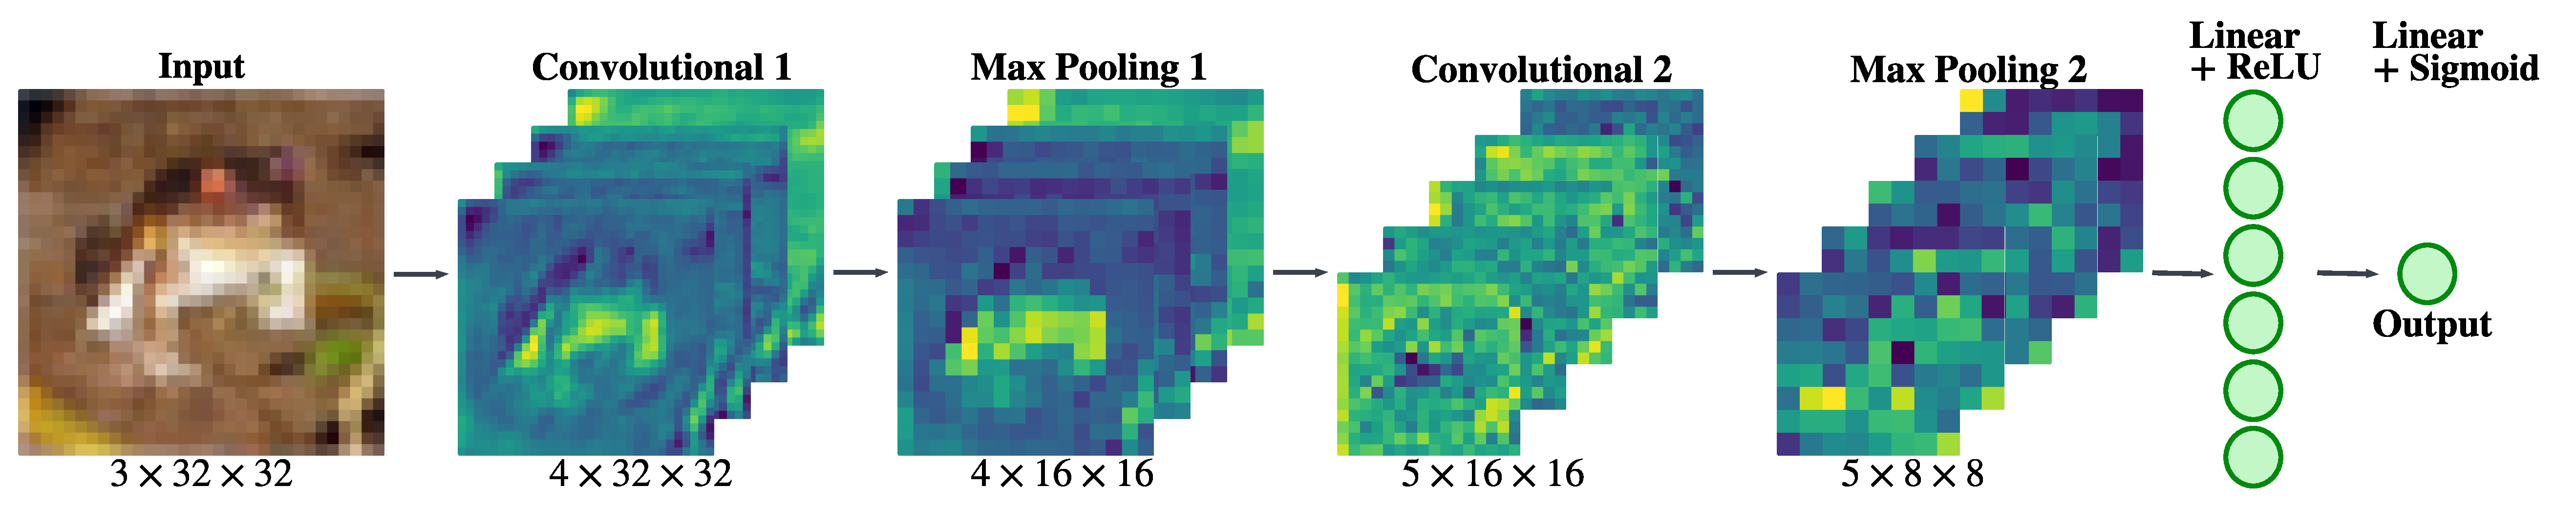
\includegraphics[width=1\textwidth]{./figures/neural_nets/CNN_frog.pdf}
    \caption{\centering A binary classification CNN processing an image of a frog.}
    \label{fig:CNN_frog}
\end{figure}

\noindent Before these deep learning architectures, researchers would have to perform feature extraction and feed the extracted feature values to a chosen model, e.g. an SVM for classification. The disadvantage of this is that one would have to pick a feature extraction method and a model to go along with it. Which feature extraction algorithms work best for a given model? This is annoying to have to do. To alleviate this, deep learning architectures streamline the process. A huge advantage is that, in some sense, these deep learning models know what features are best for the `prediction' part of the model.

So how do these earlier layers in CNN architectures perform feature extraction? Convolution and pooling layers.

\subsubsection{Convolutions}
Convolution operations involve using a square matrix to, in some sense, summarise the information embedded in the pixels it traverses over. This square matrix is called the kernel or filter (synonymous and I switch a lot). You can think of this convolution operation as a sort of dot product between the filter and the pixel values it is on top of at that point.

More formally, given a feature map $I\in\mathbb{R}^{C\times W\times H}$ and a kernel $K\in\mathbb{R}^{C\times k\times k}$ with $k<W$ and $k<H$, the feature map $F=K*I\in\mathbb{R}^{W'\times H'}$ given by the convolution of $K$ over $I$ is given by
$$
F_{i,j}
=
\sum_{c=1}^C\sum_{x=1}^{k}\sum_{y=1}^{k}K_{c,x,y}\cdot I_{c,i+x,i+y}+b_c
$$
where $b_c$ is the kernel's bias in channel $c$. Note that this notation is intended to illustrate what a convolution looks like algebraically. As it stands, what's written above does not account for padding, stride, etc. For a simpler illustration, consider \autoref{fig:convolution_operation}.

\begin{figure}[ht]
    \centering
    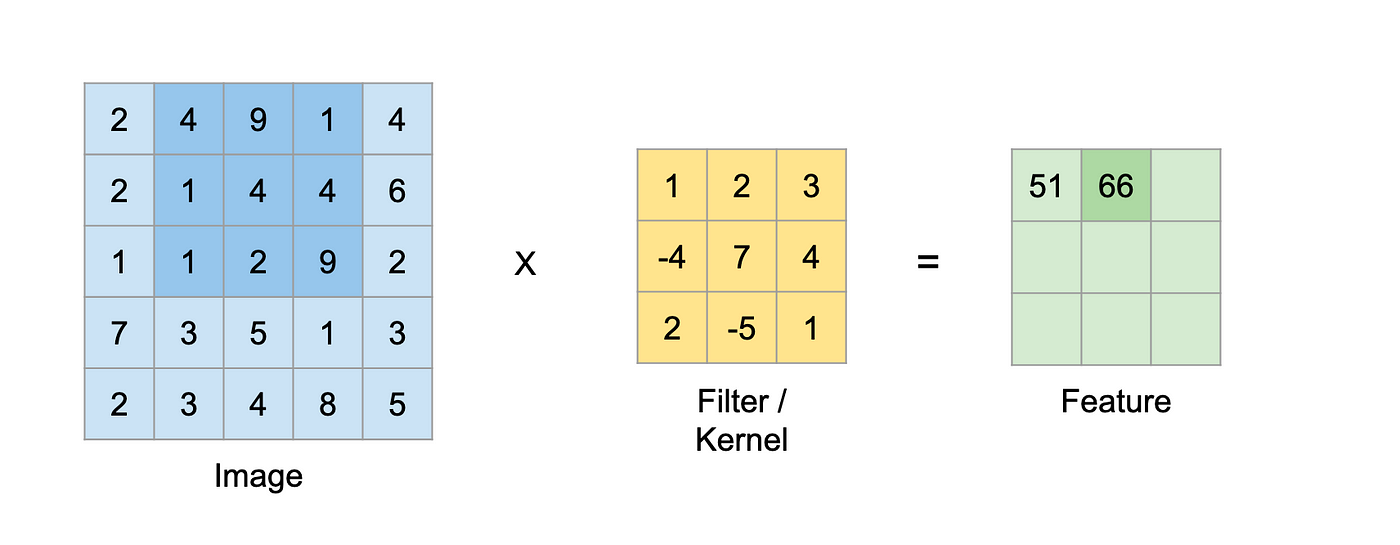
\includegraphics[width=1\textwidth]{./figures/neural_nets/convolution.png}
    \caption{\centering Convolution without bias.}
    \label{fig:convolution_operation}
\end{figure}

\noindent Generally, earlier convolutions in a CNN architecture extract higher level features, like edges and textures, while later convolutions extract lower level features that are usually beyond human interpretation. This is observed in \autoref{fig:CNN_frog} where after the first convolutional layer one can still see a resemblance of the input image of a frog. The feature maps produced by the second convolutional layer do not maintain a human interpretable resemblance of the frog.

\subsubsection{Pooling}
Pooling operations reduce the spatial dimensions of a given feature map by, in some sense, clustering certain parts of the feature map. There's not much point to writing this mathematically rigorously. Instead, consider \autoref{fig:pooling}. Pooling has a ton of flavours: max, min, average and more.

\begin{figure}[ht]
    \centering
    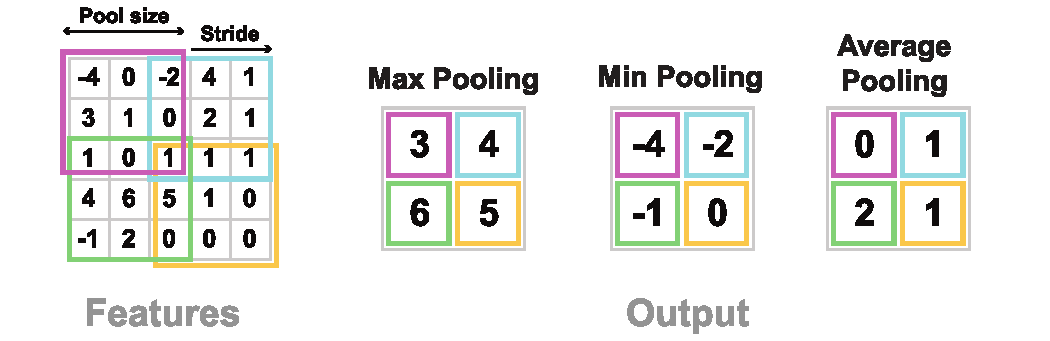
\includegraphics[width=1\textwidth]{./figures/neural_nets/pooling.pdf}
    \caption{\centering The core flavours of pooling.}
    \label{fig:pooling}
\end{figure}

\noindent I typically just pick max pooling and see how it does. A nice benefit of pooling is improved robustness to translations of images. Ideally, our model would classify an image in a similar enough way to how it'd classify the same image but slightly shifted. What is meant here is very problem-dependent so take it with a grain of salt. Hopefully the idea is clear anyway. Another core benefit is the reduced compute.

\subsubsection*{Output dimensions of convolutions and pooling}
Given a feature map $F\in\mathbb{R}^{W\times H}$, suppose we compute the convolution $O\in\mathbb{R}^{W'\times H'}$ of the kernel $K\in\mathbb{R}^{k\times k}$ over $F$ with uniform padding $P$ and stride $S$. The precise dimensions $W'$ and $H'$ of the new feature map $O$ are given by
$$
W'
=
\left\lfloor
\frac{W+2P-k}{S}
\right\rfloor
+1
$$
and
$$
H'
=
\left\lfloor
\frac{H+2P-k}{S}
\right\rfloor
+1.
$$
It's not too tricky to derive these. It's the kinda thing you do once and never again. Maybe worth mentioning that some frameworks allow going beyond the edges of a feature map when convolving, e.g. Pytorch's \texttt{MaxPool2d} has a \texttt{ceil\_mode} flag that determines whether the does precisely this.

\subsubsection{Example}
CNNs are best understood by example. Consider the nice frog in \autoref{fig:CNN_frog}. The input to the model is a $32\times32$ RBG image, so $3\times32\times32$ accounting for the three colour channels. This input is fed into the first layer of our CNN which is a convolutional layer. This convolutional layer has 32 filters/kernels each of which is $3\times3\times3$. I prefer to think of each of these kernels as three separate $3\times3$ kernels, one for each colour channel. For a given kernel triplet, each is slid over the $32\times32$ image corresponding to their channel, each yielding a $30\times30$ output. Since each kernel triplet outputs three such $30\times30$ outputs, we sum them to obtain the overall feature map corresponding to this kernel.

There are 32 kernel triplets in our case and so you can think of the output of this layer as 32 images each of which are $30\times30$ in spatial dimension. Alternatively, you can think of the output as a single tensor of dimensions $32\times30\times30$. Also, each is passed through a non-linear activation function purely for the purpose of sprinkling in some non-linearity.

% recurrent neural networks
\subsection{Recurrent Neural Networks (RNNs)}
\dots

\subsubsection{Long Short-Term Memory (LSTMs)}
\dots

\subsubsection{Gated Recurrent Units (GRUs)}
\dots

% autoencoders
\subsection{Autoencoders}
\label{sec:autoencoders}
Autoencoders are a nice precursor to variational autoencoders (VAEs). Essentially, autoencoders are neural nets in which you have a bottleneck layer in the middle of the network which compresses inputs in a way that allows for the reconstruction after decoding. So an encoder can be written as a function $\mathcal{E}:\OX\rightarrow\R^d$. Similarly, a decoder can be written as a function $\D:\R^d\rightarrow\OX$. Ideally, for all $\x\in\X$ we have $\D(\mathcal{E}(\x))=\x$ but of course in practice it is only practical to achieve $\D(\mathcal{E}(\x))\approx\x$.

\begin{figure}[ht]
    \centering
    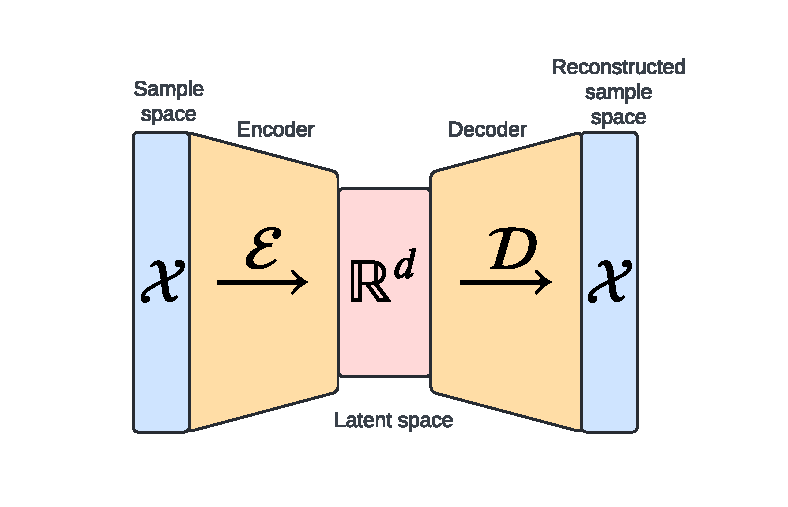
\includegraphics{./figures/neural_nets/autoencoder.pdf}
    \caption{\centering An autoencoder mapping from the sample space $\OX$ to the latent space $\R^d$ then back to $\OX$.}
    \label{fig:autoencoder}
\end{figure}

The encoder architecture is typically pretty straightforward: some neural net with an input layer consisting of a number of neurons that matches the dimension of $\OX$, some hidden layers and an output layer with $d$ neurons matching the dimension of the latent space $\mathbb{R}^d$. Similarly, the decoder architecture consists of an input layer of $d$ neurons, some hidden layers and an output layer of $\text{dim}(\OX)$ neurons. So the idea is simple: train the encoder $\mathcal{E}$ and decoder $\D$ such that $\D(\mathcal{E}(\x))\approx\x$ for all $\x\in\OX$ where $\text{dim}(\text{Im}(\mathcal{E}))<<\text{dim}(\OX)$.

\subsubsection{Example autoencoder (visualisation bonus)}
Consider the MNIST dataset, bunch of handwritten digits. Let's learn an autoencoder in which the latent space is $\R^2$. A nice advantage of picking latent spaces whose dimension is $1$, $2$ or $3$ is that we can visualise the mappings of samples in $\OX$ to the latent space and see if there is some structure there, e.g. we can inspect if it separate them nicely.

Our encoder architecture will have an input layer consisting of 784 nodes, matching the size of samples in MNIST, two hidden layers of ? neurons each and an output layer consisting of two nodes (tight bottleneck). The decoder will then have an input layer of two nodes, two hidden layers of ? neurons each and an output layer consisting of 784 nodes.

% skip connections
\addtocontents{toc}{\protect\setcounter{tocdepth}{1}}
\subsection{Skip Connections/Residual Networks}
\addtocontents{toc}{\protect\setcounter{tocdepth}{2}}
\begin{itemize}
    \item Most intuitive benefit: it helps prevent some layer in the architecture from degrading the input entirely. It's like a nice reminder to the model what it was working from before it got to this point
    \item Reduces vanishing or exploding gradients - opens the door to far deeper architectures
    \item Ensures that the model has to learn the residual as opposed to the full underlying function: faster convergence usually
    \item Takes pressure off parameter initialisation - if you set parameters to zero then initially model is just identity and learning from their is feasible
\end{itemize}

% misc. questions
\addtocontents{toc}{\protect\setcounter{tocdepth}{1}}
\subsection{Misc. questions}
\addtocontents{toc}{\protect\setcounter{tocdepth}{2}}

Some questions to challenge one's understanding.

\begin{center}
    \textbf{\textcolor{blue}{Q1:} How does one prevent overfitting in NNs?}
\end{center}
\textbf{Early stopping -} Split training into training and validation sets. After each epoch (or every few), compute both training and validation losses. If training loss is decreasing while validation loss is not decreasing then you're at risk of overfitting. For illustration, consider \autoref{fig:early_stopping} in which the training loss continues to decrease in the number of epochs while the validation loss seems to reach its lowest value around epoch 28.

\begin{figure}[ht]
    \centering
    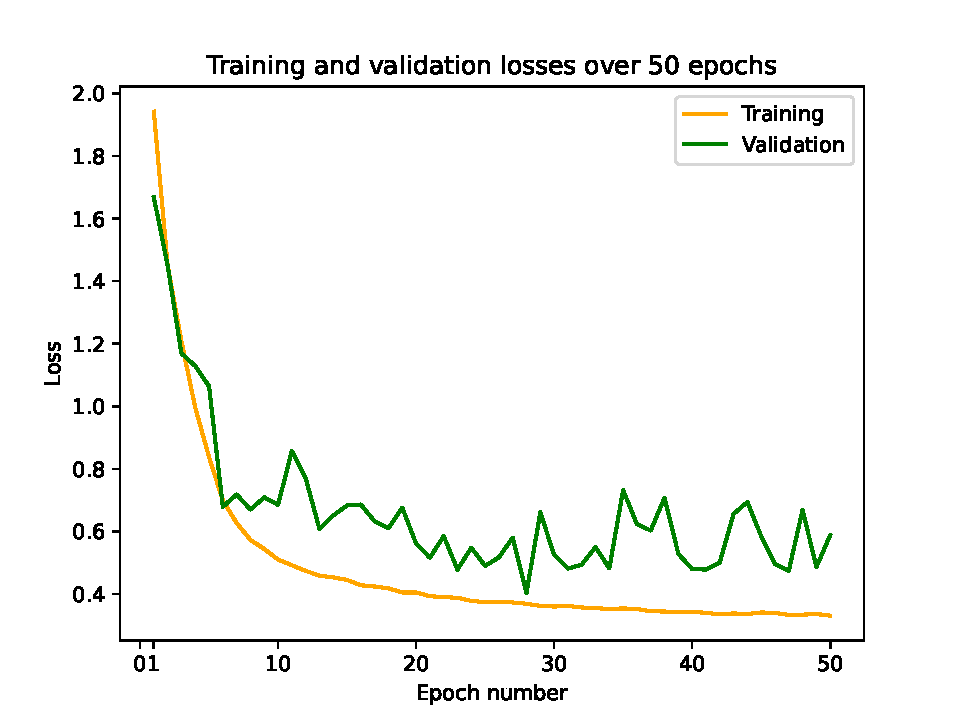
\includegraphics[width=0.5\textwidth]{./figures/neural_nets/early_stopping.pdf}
    \caption{Training and validation losses over 50 epochs for some model.}
    \label{fig:early_stopping}
\end{figure}

\noindent If you observe this for sufficiently many consecutive epochs then you can stop training and use the parameters pertaining to the epoch at which the validation loss was lowest. To do this, at each epoch during training, save the parameters of the current epoch if they offer a lower validation loss than at any epoch before. This is often referred to as a checkpoint within the training process and the parameters are saved in a \texttt{.ckpt} file.\\

\noindent\textbf{Dropout -} We don't want to be overly-reliant on any given subset of neurons. To prevent such dependencies, at each epoch, independently set the activation of each neuron to 0 with probability $p$. This way some portion of neurons are silenced during the training epoch. As a result, its corresponding parameters (weights and bias) are not updated during backpropagation - it is truly silenced. This idea is illustrated in \autoref{fig:dropout}. Do not perform dropout when testing.

\begin{figure}[ht]
    \centering
    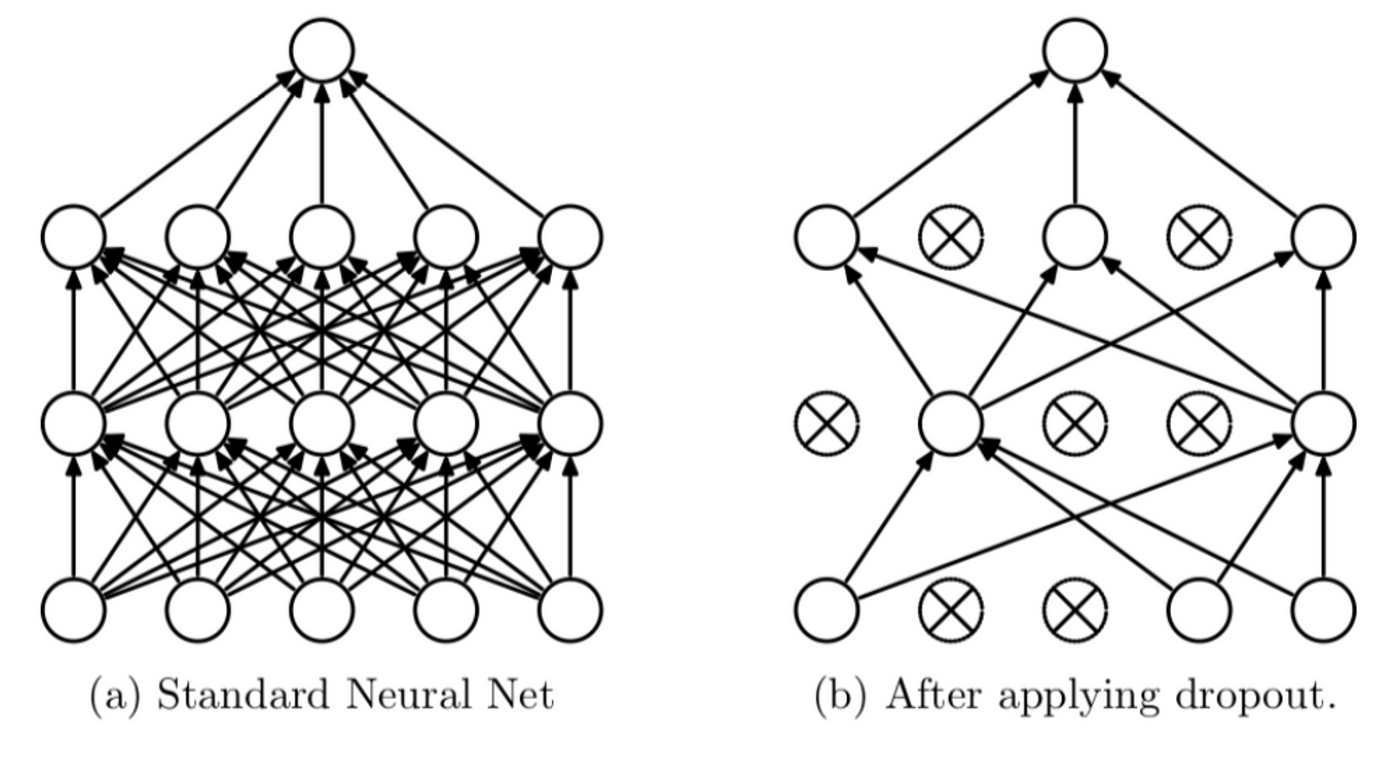
\includegraphics[width=0.5\textwidth]{./figures/neural_nets/dropout.png}
    \caption{Dropout to prevent overdependence.}
    \label{fig:dropout}
\end{figure}

\begin{center}
    \textbf{\textcolor{blue}{Q2:} What is the purpose of activation functions?}
\end{center}
Without the application of at least one activation function, the values of the output neurons would simply be the result of matrix-vector multiplication and vector addition. That is to say, the output of the neural network, without an any activation function, would be a purely linear transformation of the input. The issue with this is that most problems require some degree of non-linearity. The staple example of this is the classification of two-dimensional samples which are not linearly-separable.

\begin{figure}[ht]
    \centering
    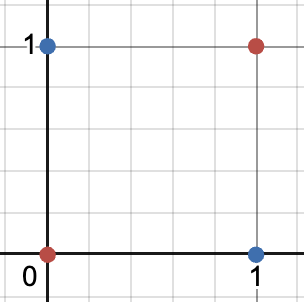
\includegraphics[width=0.40\columnwidth]{./figures/neural_nets/xor.png}
    \hspace{20pt}
    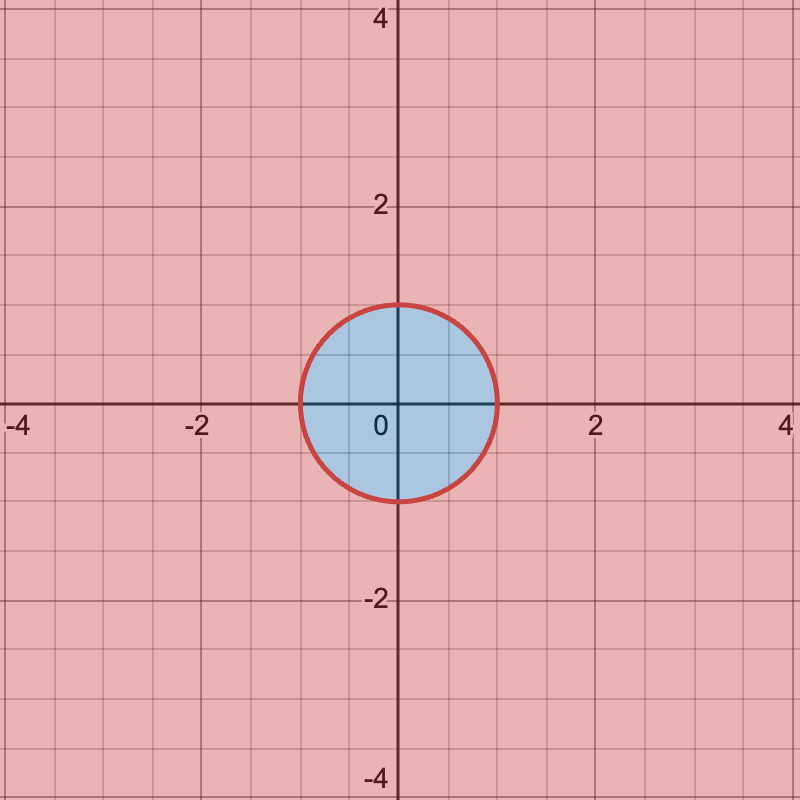
\includegraphics[width=0.40\columnwidth]{./figures/neural_nets/circle.png}
    \caption{\centering Examples of samples belonging to classes that are not linearly-separable.}
    \label{fig:non_linearly_separable}
\end{figure}

\noindent The point is that there is no line that would separate the classes in either case: non-linearity is needed! In the latter case, it is desirable to be able to somehow punch the interior of the unit disc to form a blue mountain with the surrounding ground covered in red. This can be achieved by the non-linear transformation $\phi(x,y)=\max(0,1-(x^2+y^2))$ which is illustrated in \autoref{fig:non_lin_transformation}.

\begin{figure}[ht]
    \centering
    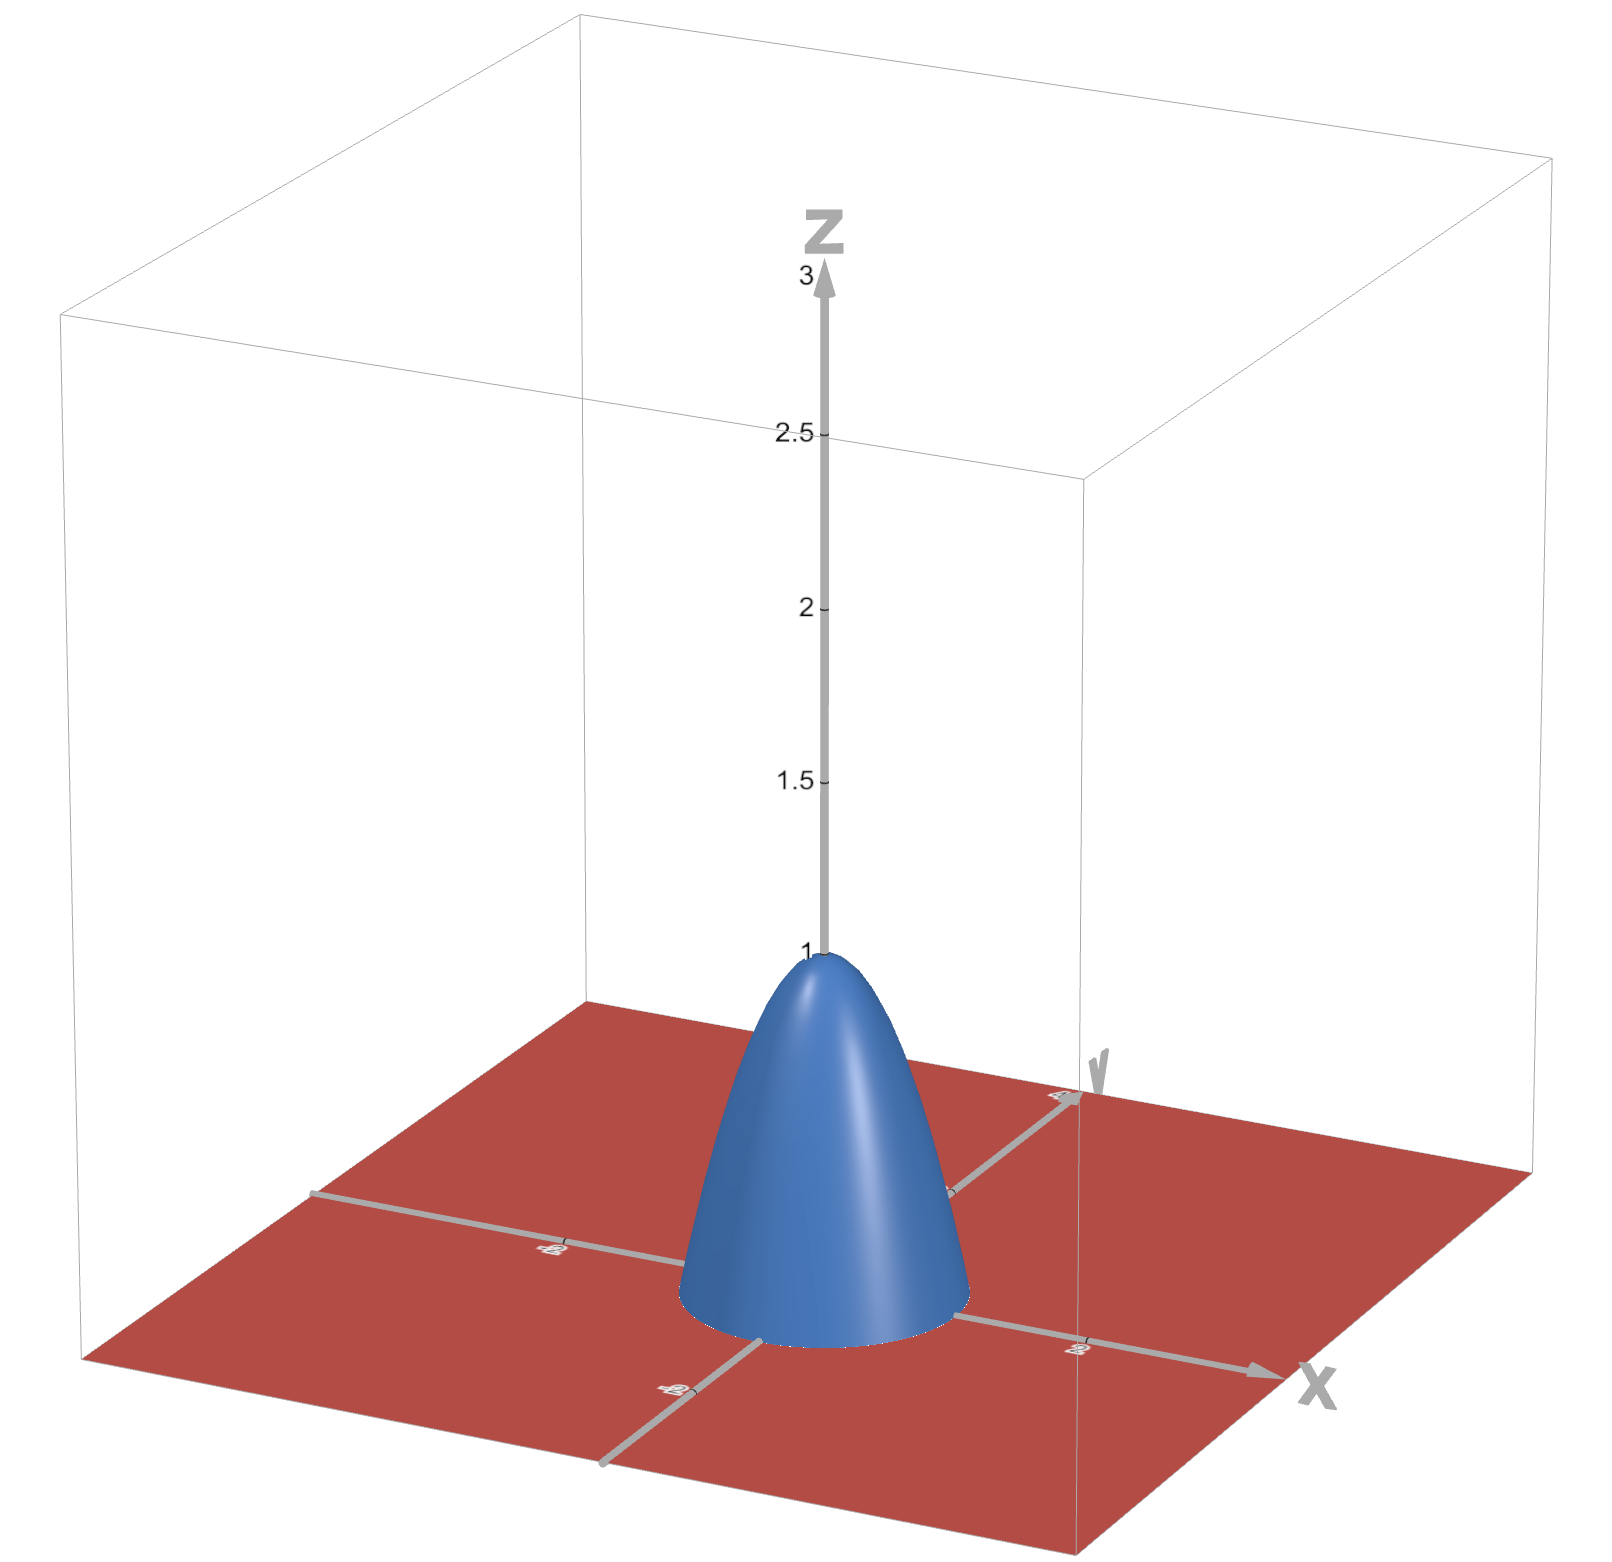
\includegraphics[width=0.40\columnwidth]{./figures/neural_nets/non_lin_transform.png}
    \caption{\centering The image of our non-linear transformation.}
    \label{fig:non_lin_transformation}
\end{figure}

From here, a natural linear decision boundary is just the plane $z=0$. Any sample above the plane, i.e. any sample whose $z-$coordinate is positive, is classified as blue. It is otherwise classified as red. We can be more clever than this though. This transformation required us to map samples to 3D - how about mapping to just 1D? To do this, a complete decision function is given by $D(x,y)=\left\lceil\frac{\left\lfloor x^2+y^2\right\rfloor}{x^2+y^2}\right\rceil$ and just define $D(0,0)=0$ to avoid the annoying pole.

\begin{center}
    \textbf{\textcolor{blue}{Q3:} Why not just one activation function in the output layer?}
\end{center}
If there were a single activation function towards the end of the architecture then everything that came before would be a series of linear transformations of the input. The composition of linear transformations is just a linear transformation. As such, the model would effectively be a single linear layer into a non-linear transformation. The only way this could be effective would be if the non-linear transformation were effectively the function we're looking to model in the first place.

\textcolor{red}{note that this is just a single-layer perceptron}: most activation functions are monotonic, so SLPs reduce to, again, a hyperplane in feature space. like the first paragraph states, if we allow for arbitrary non-linear activation functions then this is possbile in theory (but unrealistic). monotonicity kills it

\begin{center}
    \textbf{\textcolor{blue}{Q4:} Must activation functions be monotonic?}
\end{center}
No, just makes it much easier to optimise when they are.

\begin{center}
    \textbf{\textcolor{blue}{Q5:} Which activation functions should be used when?}
\end{center}
Roughly speaking, I wouldn't worry too much about this in practice. They're all nice and differentiable (with small caveats here and there, like with ReLU) allowing for the application of backpropagation. You should sometimes care about the output given the problem at hand. For example, if you need outputs in $[-1,1]$ then $\tanh$ is a natural choice. Note that some choices, like Leaky ReLU, introduce hyperparameters to the model which is sometimes undesirable, e.g. if one seeks a hyperparameterless model.

Small fun note, the universal function approximation of MLPs has been proven only for some select activation functions. I should look in more detail about this.

\begin{center}
    \textbf{\textcolor{blue}{Q6:} Why use a CNN over an MLP?}
\end{center}
Suppose we have an MLP and a CNN, both trained to perform binary classification on images of cats and dogs. Further, suppose they perform equally. It might not be too surprisnig that the MLP will necessarily consist of a number of parameters that is orders of magnitude greater than for the CNN. Also, it's not so clear if a given MLP is translation invariant while various components of a CNN architecture help alleviate fears of translation-related issues.

On top of this, pixel values are very usually correlated, so why use an MLP in which many nodes are redundant? CNN's take care of this perfectly. They were handcrafted for processing image data and so they are naturally far superior. 

% generative models
\newpage
\section{Generative Models}

Since the era of deep learning began in 2012, tons of generative image, video and text models have arisen. The general idea of these generative models is that if we have a model that fits training data particularly well then samples from the model should be sufficiently convincing. That is, if I get a nice fit for the distribution of images of cats lounging in the sun then samples from my fit distirubtion should look convincingly like cats lounging in the sun.

The problem with fitting such a distribution is that it is not at all clear what the distribution function would be. These distributions are complex and generally very hard to get right. Most ways to fit the underlying distribution is to perfrom maximum likelihood in some way. Performing maximum likelihood directly without access to any sort of direct distribution function is pretty hard, so it is often done indirectly. For example, when training a variatioanl autoencoder (VAE), you look to maximise a lower bound of the likelihood. The idea is that if this lower bound is sufficiently tight then maximising it in some sense pushes up the true likelihood, maximising it.

% variational autoencoders
\subsection{Variational Autoencoders (VAEs)}
In \autoref{sec:autoencoders}, autoencoders (AEs) were discussed. Autoencoders are great for data compression/decompression, denoising, interpreting complex models, etc. but we haven't seen yet how we might make use of them for generative tasks, i.e. sampling from the nasty/complex underlying distribution of the data they are trained on. An intuitive first idea is to train a compression/decompression autoencoder, randomly generate points in its latent space and feed them through the decoder, as in \autoref{fig:autoencoder_generation_1}. The outputs of the decoder should be similar to the training data, right? No.

\begin{figure}[ht]
    \centering
    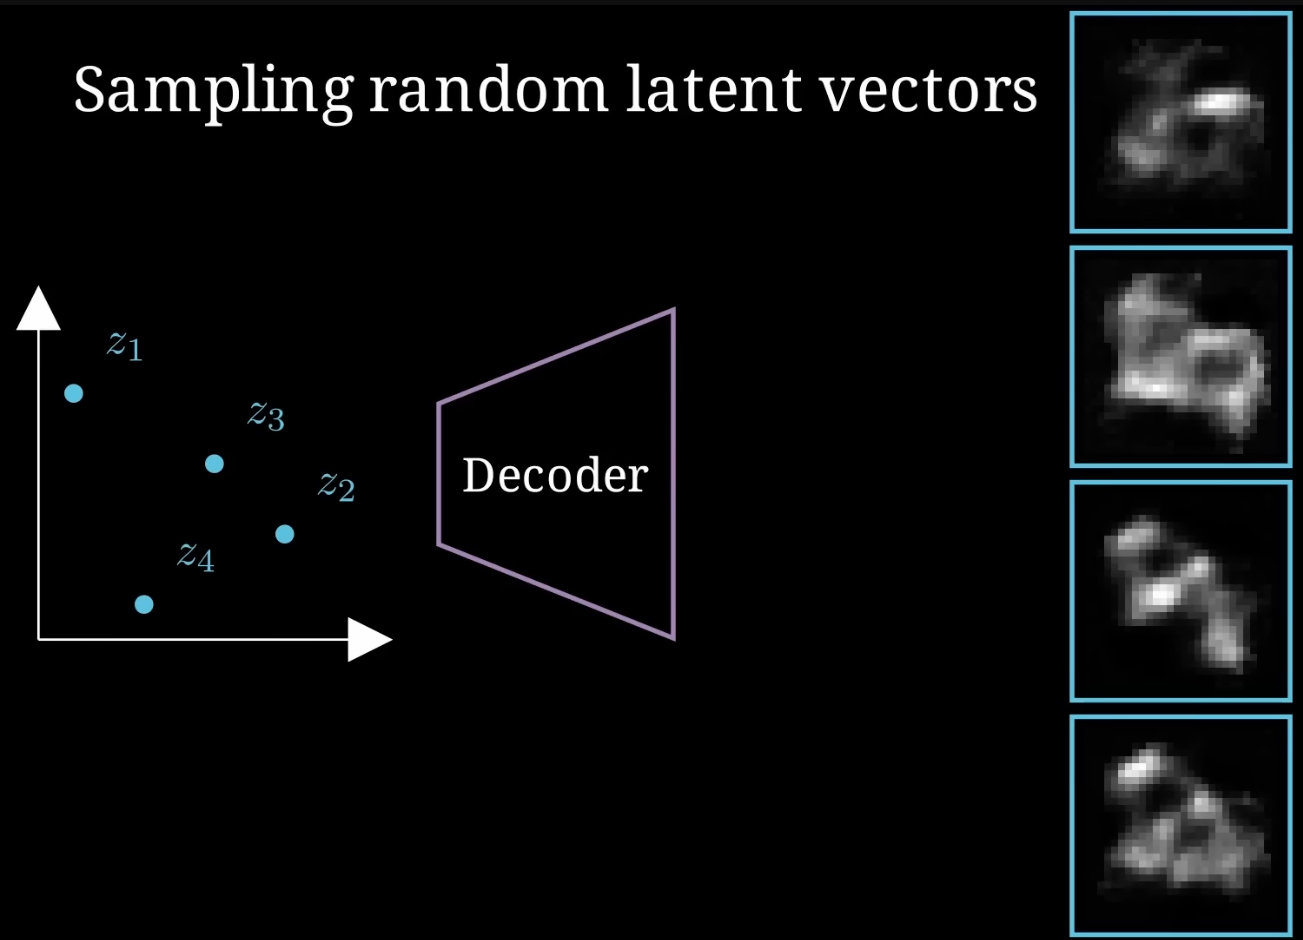
\includegraphics[width=0.60\columnwidth]{./figures/generative_models/AEs_gen_1.png}
    \caption{\centering The output of the decoder of an autoencoder with randomly generated latent points as input. Gibberish output.}
    \label{fig:autoencoder_generation_1}
\end{figure}

Disaster strikes and we begin to see just how unstructured the latent space of an autoencoder is: randomly sampling from it (whatever this may mean) results in nonsense outputs from the decoder because most of the latent space itself is meaningless (nothing is encoded to most of it, so in some sense a lot of it is `un-utilised'). This is perhaps unsurprising as at no point during training an autoencoder do we impose any sort of restriction on the structure of its latent space.

New idea: how about we feed the decoder latent points that are pretty close to the embedding of a given training sample, as in \autoref{fig:autoencoder_generation_2}? This should result in decoder outputs that are similar in structure to the input sample but a bit different, right? No.

\begin{figure}[ht]
    \centering
    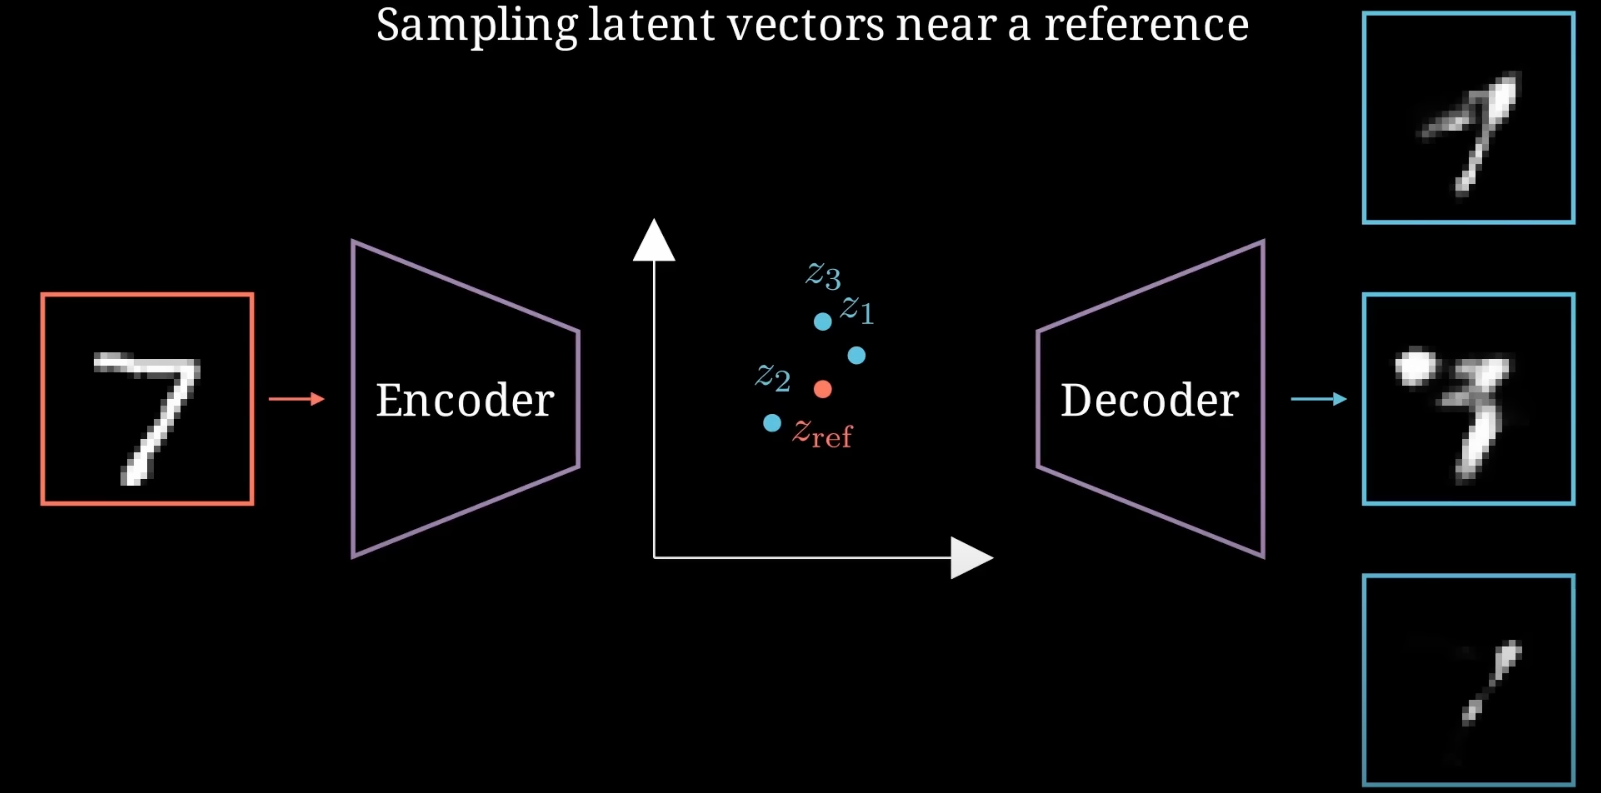
\includegraphics[width=0.75\columnwidth]{./figures/generative_models/AEs_gen_2.png}
    \caption{\centering The output of the decoder of an autoencoder points relatively close to the latent embedding of a given training sample.}
    \label{fig:autoencoder_generation_2}
\end{figure}

Distaster strikes again. To get decoder outputs that are meaningful using this idea, one must take points in the latent space which are ridiculously close to this chosen sample's latent embedding. So close that you'd be practically reconstructing the original training sample each time - certainly not what we mean when we say that we'd like to generate samples.

Queue variational autoencoders (VAEs), illustrated in \autoref{fig:VAE_architecture}. Loosely put, they have a somewhat similar structure to regular autoencoders in that they have an encoder and a decoder but they are distinguished by two things. First, they impose structure on the latent space which helps very much with making the ideas presented earlier feesable. For example, points that are close in feature space are also close in the latent space and all of the latent space is made use of, none of it meaningless. Second, given fixed inputs, the outputs of the encoder and decoder are not fixed points (hence variational). Instead, the outputs are parameters of sampleable distributions.

\begin{figure}
    \centering
    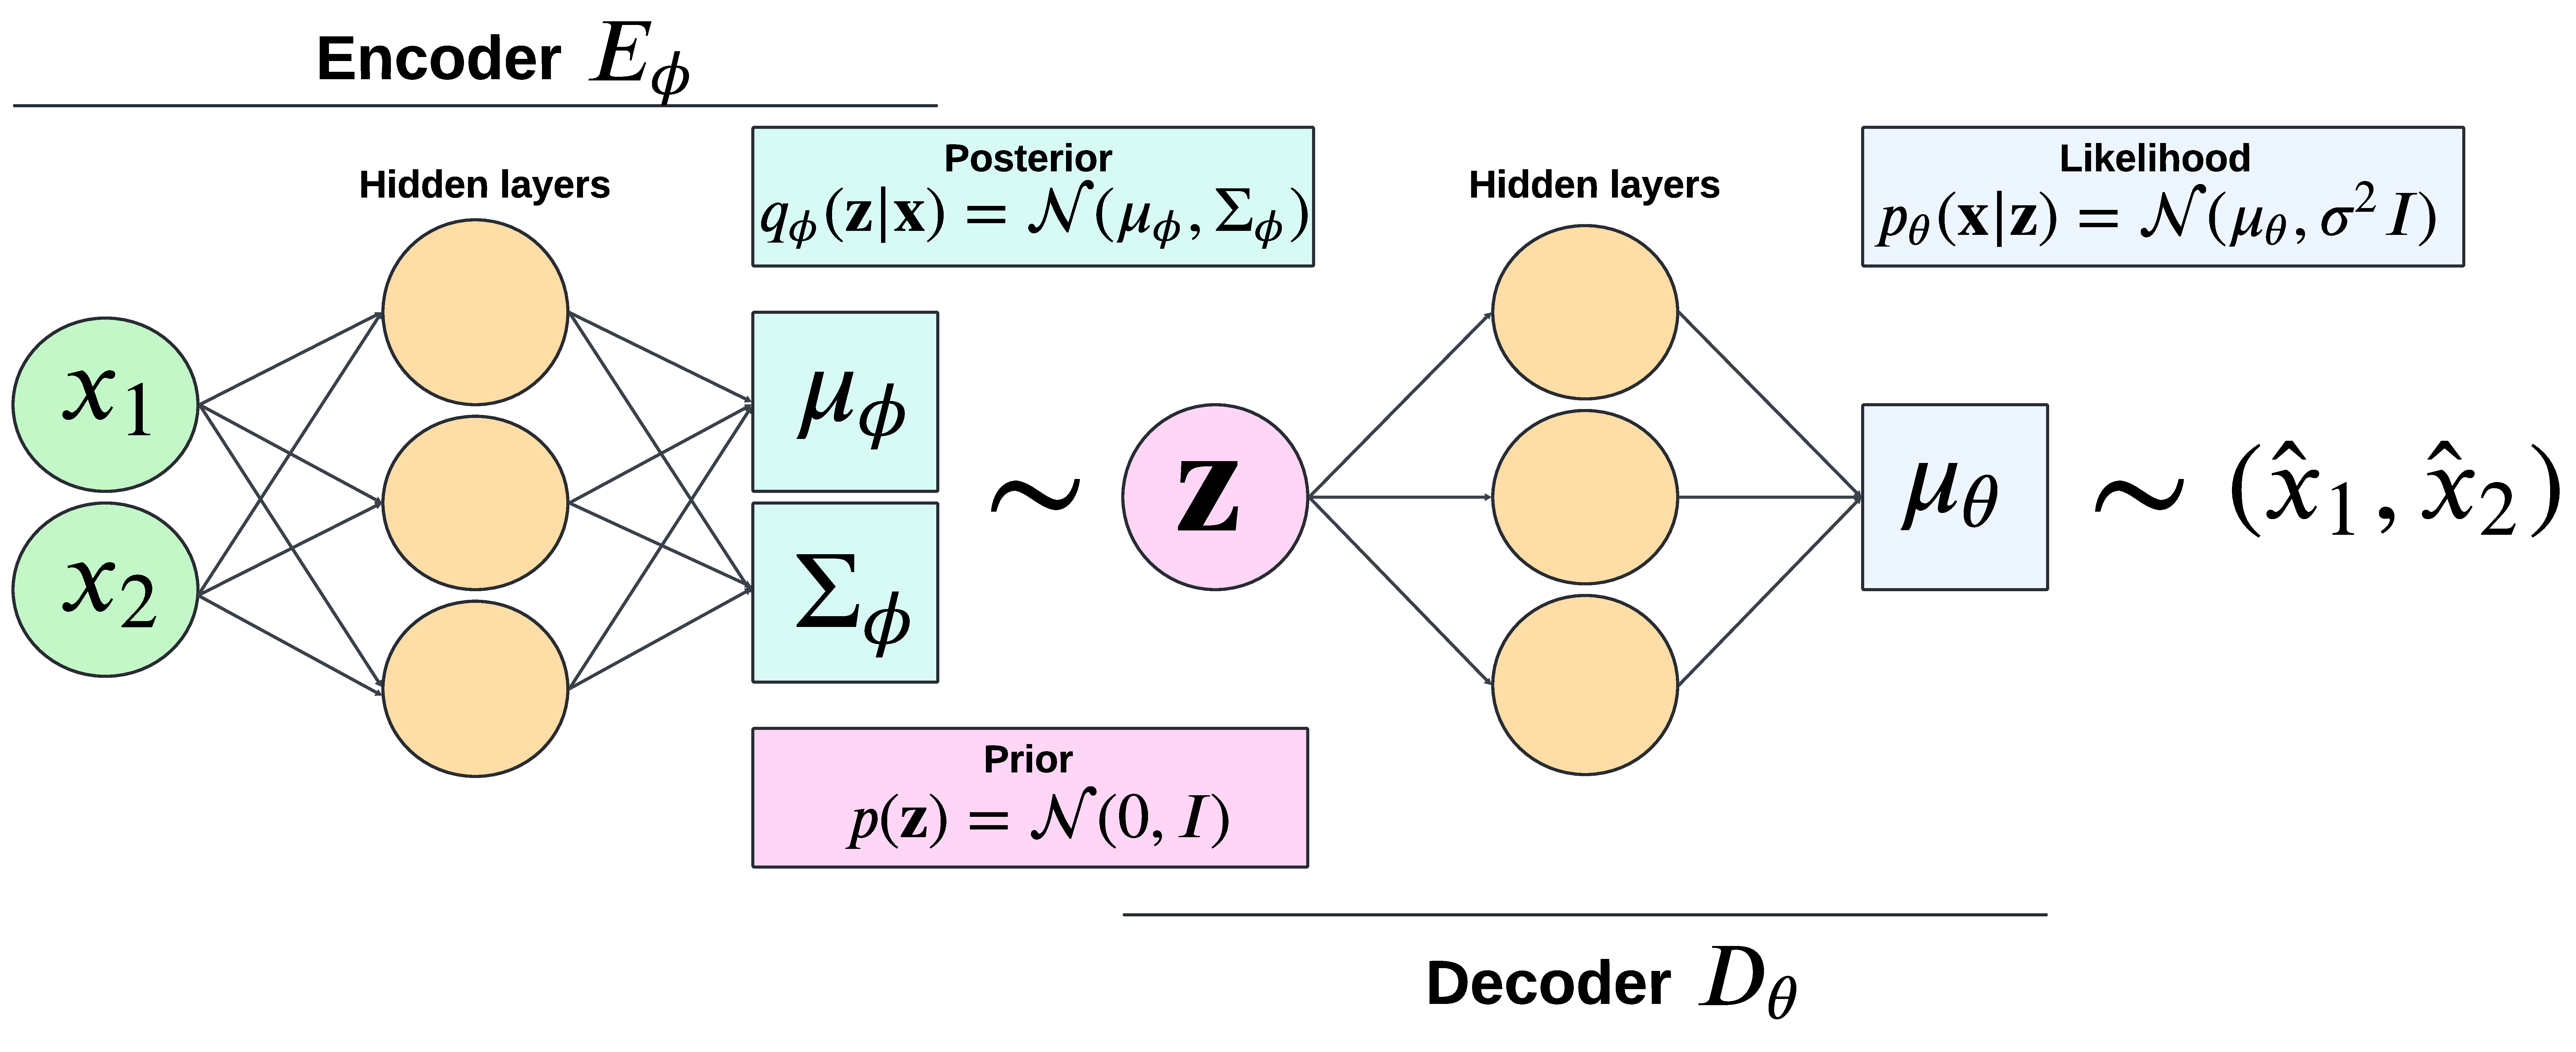
\includegraphics[width=1\columnwidth]{./figures/generative_models/VAE_handcrafted.pdf}
    \caption{\centering Example architecture of a variational autoencoder in which the input distribution is two-dimensional.}
    \label{fig:VAE_architecture}
\end{figure}

\subsubsection{think of different subsubsection name}
Denote the parameters of the encoder by $\phi$ and the paramaters of the decoder by $\theta$. Note that sometimes I will write $\phi(\x)$ to denote the output of the encoder, which is a little odd as $\phi$ denotes the encoder's paramteres but it makes notation a little easier. Anyway, the role of the encoder and decoder in VAEs is to output paramters of sampleable distributions. For example, in the vanilla formulation, a VAE's encoder takes in some sample $\x$ and outputs the parameters $\mu_{\phi}$ and $\Sigma_{\phi}$ (usually diagonal) of a normal distribution which approximates the posterior distriubtion $\Z|\x$. If we want to reconstruct $\x$, we sample from $q_{\phi}(\z|\x)=\N(\mu_{\phi}, \Sigma_{\phi})$ and feed it as input to the decoder which outputs the mean $\mu_{\theta}$ of $p_{\theta}(\x|\z)=\N(\mu_{\theta},\sigma^2 I)$ where $\sigma$ is a hyperparameter. Sampling from this approximation of the likelihood distribution $\X|\z$ will yield something close to $\x$ itself.

While the idea itself is clear, the difficulty in having it come to fruition is training such an architecture, i.e. finding the parameters $\phi$ and $\theta$ that offer the best reconstruction and smooth latent space, all according to some metric. In line with most other approaches to generative modelling, if we can do maximum likelihood in some way, i.e. ensure that the likelihood of the training data is maximal under our model then samples from the likelihood distribution, whose parameters are output by the model's decoder, should resemble those in the training set. To do this, we would ideally perform maximum likelihood directly but we don't have access to the true underlying joint distribution function $p(\x)$. As such, we instead look to find a lower bound for $p(\x)$ which we maximise instead. The idea is that pushing this supposed lower bound up will in turn push up $p(\x)$ itself. In line with this, we derive the evidence lower bound (ELBO), first noting that
$$
p(\x)
=
\int p(\x,\z)d\z
=
\int p(\x|\z)p(\z)d\z
\approx
\int p_{\theta}(\x|\z)p(\z)d\z
$$
where the parameters of $p_{\theta}(\x|\z)$ are given by VAE's decoder. Note that an almost identical method can be used for discrete random variables, integrals just look prettier. From here, we can utilise Jensen's inequality to obtain
\begin{align*}
    \log(p(\x))
    &=
    \log\left(\int p_{\theta}(\x|\z)p(\z)d\z\right)\\
    &=
    \log\left(\int q_{\phi}(\z|\x)\frac{p_{\theta}(\x|\z)p(\z)}{q_{\phi}(\z|\x)}d\z\right)\\
    &=
    \log\left(\E_{q_{\phi}(\z|\x)}\left[\frac{p_{\theta}(\x|\Z)p(\Z)}{q_{\phi}(\z|\x)}\right]\right)\\
    &\geq
    \E_{q_{\phi}(\z|\x)}\left[\log\left(\frac{p_{\theta}(\x|\Z)p(\Z)}{q_{\phi}(\Z|\x)}\right)\right]\\
    &=
    \E_{q_{\phi}(\z|\x)}\left[\log(p_{\theta}(\x|\Z))\right]-\E_{q_{\phi}(\z|\x)}\left[\log\left(\frac{q_{\phi}(\Z|\x)}{p(\Z)}\right)\right]\\
    &=
    \E_{q_{\phi}(\z|\x)}\left[\log(p_{\theta}(\x|\Z))\right]-D_{\text{KL}}(q_{\phi}(\Z|\x)||p(\Z))\\
    &=:
    \text{ELBO}
\end{align*}
where the parameters of $q_{\phi}(\z|\x)$ are given by the VAE's encoder. As such, for a training set $\{\x_i\}_{i=1}^N$, we look to compute

$$
\argmax_{\phi,\theta}\sum_{i=1}^N\left[\E_{q_{\phi}(\z|\x_i)}\left[\log(p_{\theta}(\x_i|\Z))\right]-D_{\text{KL}}(q_{\phi}(\Z|\x_i)||p(\Z))\right].
$$
If we can maximise the ELBO then we are doing some sort of pseudo-maximum likelihood but what do the individual terms mean? The first term, $\E_{q_{\phi}(\z|\x)}\left[\log(p_{\theta}(\x|\Z))\right]$ pertains to how well the model reconstructs an input $\x$ given its latent representation. The motive of maximising this is self-explanatory. The second term, however, isn't entirely clear at first and motivations for minimising it are usually pretty bad. Minimising the KL-divergence term $-D_{\text{KL}}(q_{\phi}(\Z|\x)||p(\Z))$ pertains to encouraging our approximation of the posterior to be close to our chosen prior (usually just $\N(0,I)$). There is good reason to desire this as any usual choice of prior is nicely structured. It ensures that sampling from the prior distribution is sufficiently similar to sampling from the posterior itself. Note that more often than not, even though this ensures that the posterior is well-structured, this does not mean that it looks human-interpretable\footnote{\url{https://n8python.github.io/mnistLatentSpace/}}.

It turns out that the ELBO is a very tight bound in many cases - even to the extent of performing very well on density estimation benchmarks.

\subsubsection{The Reparameterization Trick}
Back propping through sampling is not a thing, it ain't differentiable 

\subsubsection{VAE architecture for MNIST}
For generating new sample of MNIST, the following architecture worked for me. Encoder:
\begin{itemize}
    \item three hidden layers of $h/4$, $h/2$ and $h$ neurons respectively where $h=4096$ is the hidden dimension
    \item ReLU for each hidden layer and just linear maps for parameters
    \item a latent dimension of $256$
\end{itemize}

% general adversarial networks
\subsection{Generative Adversarial Networks (GANs)}
Compete!

% normalising flow models
\subsection{Normalising Flow Models}
Turn noise to samples!

% diffusion models
\subsection{Diffusion Models}
Turn noise to samples!

% transformer models
\subsection{Transformers}
Stand at attention!

\subsubsection{Token embedding}
Embed the semantics of tokens in high-dimensional space. ``Germany" plus ``fascist" minus ``Mussolini" equals ``Hitler".

\subsubsection{Positional encoding}
Use sinusoids to form a position vector $P_k$ for the $k$th token in an input sequence of length $L$. Add $P_k$ to the word embedding $E_k$ for $k=0,\dots,L-1$ to obtain the input $[E_0+P_0,\dots,E_{L-1}+P_{L-1}]$ fed to the model.

% misc. questions
\addtocontents{toc}{\protect\setcounter{tocdepth}{1}}
\subsection{Misc. questions}
\addtocontents{toc}{\protect\setcounter{tocdepth}{2}}

Some questions to challenge one's understanding.

\begin{center}
    \textbf{\textcolor{blue}{Q1:} Why choose normal priors in VAEs?}
\end{center}
\dots

% appendices
\newpage
\begin{appendices}
\addtocontents{toc}{\protect\setcounter{tocdepth}{0}}

% probability things
\section{Probability Theory Things}

\begin{tcolorbox}[colback=c5]
    \textbf{Discrete:}
    \begin{itemize}
        \item Poisson, Geometric $\rightarrow$ Negative Binomial \textbf{(generic)}
        \item Bernoulli $\rightarrow$ Binomial \textbf{(binary classification)}
        \item Categorical $\rightarrow$ Multinomial \textbf{(multi-class classification)}
    \end{itemize}
\end{tcolorbox}

\begin{tcolorbox}[colback=c9]
    \textbf{Continuous:}
    \begin{itemize}
        \item Uniform, (Multivariate) Normal, Exponential \textbf{(generic)}
        \item (Multivariate) Student's $t$, Chi-squared \textbf{(classical stats)}
        \item Beta, Gamma, Dirichlet \textbf{(Bayesian stats)}
    \end{itemize}
\end{tcolorbox}

\subsection{From Bernoulli to Binomial}
Let's try to generalise the Bernoulli distribution to the binomial distribution. If $X\sim\text{Ber}(p)$ then $\Omega_X=\{0,1\}$ and $\P(X=x)=p^x(1-p)^{1-x}$, so $\P(X=1)=p$ and $\P(X=0)=1-p$.

Taking $n$ independent Bernoulli trials and summing them yields the random variable $\X=\sum_{i=1}^nX_i\sim\text{Bin}(n,p)$ with $\OX=\{0,\dots,n\}$. Let $k$ denote a realisation of $\X$, i.e. $k=x_1+\dots+x_n$. The distribution function of $\X$ is given by
\begin{align*}
    \P(\X=k)
    &=
    Z\cdot\prod_{i=1}^n\P(X_i=x_i)\\
    &=
    Z\cdot\prod_{i=1}^np^{x_i}(1-p)^{1-x_i}\\
    &=
    Z\cdot p^{x_1+\dots+x_n}(1-p)^{n-(x_1+\dots+x_n)}\\
    &=
    Z\cdot p^k(1-p)^{n-k}
\end{align*}
where $Z$ is a normalising constant accounting for the number of ways one can permute the tuple of realisations $(x_1,\dots,x_n)$. So $Z$ is just the number of ways of placing $k$-many $1$s among a series of $n>k$ digits, i.e. $Z=\binom{n}{k}$, so
$$
\P(\X=k)
=
\binom{n}{k}p^k(1-p)^{n-k}.
$$

\subsection{From Categorical to Multinomial}
The categorical distribution is a generalisation of the Bernoulli distribution and the multinomial distribution is a generalisation of the binomial distribution. As such, we'd hope to be able to generalise the categorical distribution to the multinomial distribution.

If $X\sim\text{Cat}(p_1,\dots,p_C)$ then realisations of $X$ can be represented by single integers in $\{1,\dots,C\}$ but I prefer to represent them in terms of their $C-$long one-hot encodings. So I denote the presence of the $c^{\text{th}}$ class in a realisation as the unit row vector $\mathbf{e}_c^{\text{T}}$, e.g. $(0,1,0\dots,0)$ denotes a sample in which the second class is present. The distribution function of $X$ is then given by
$$
\P(X=(x_1,\dots,x_C))
=
\prod_{j=1}^Cp_j^{x_j}.
$$
Note that, in this notation, all but one of these $x_j$ terms are zero, so it really boils down to just a single probability value, e.g. $\P(X=(0,1,\dots,0))=p_2$. The distribution function can also be written using indicator functions but this form is easiest to understand for me.

% this needs some cleaning, the idea is good
Applying the same idea used to generalise Bernoulli to binomial, consider the random variable $\X=\sum_{i=1}^nX_i$ pertaining to $n$ independent categorical trials. Each realisation of $X_1,\dots,X_n$ can be represented by a $C-$long one-hot encoded vector and so $n$ realisations of $X\sim\text{Cat}(p)$ can be thought of as a matrix $\x\in\{0,1\}^{n\times C}$ whose rows are realisations of a categorical distribution with $C$ classes. As such, letting $k_1,\dots,k_C$ denote the number of $1$s in the columns of $\x$ (so $k_1+\dots+k_C=n$) we see immediately that $(k_1,\dots,k_C)$ is a realisation of $\X$. So what is the distribution function of $\X=\sum_{i=1}^nX_i$ with $X_1,\dots,X_n\sim\text{Cat}(p_1,\dots,p_C)$? Let $x_{ij}$ denote the element in the $i^{\text{th}}$ row and $j^{\text{th}}$ column of $\x$ and let $k_j=x_{1j}+\dots+x_{nj}$ denote the sum of all elements in the $j^{\text{th}}$ column of $\x$. Note that $k_j$ is the number of realisations of $X_1,\dots,X_n$ in which the $j^{\text{th}}$ class is present. We have
\begin{align*}
    \P(\X=(k_1,\dots,k_C))
    &=
    Z\cdot\prod_{i=1}^n\P(X_i=(x_{i1},\dots,x_{iC}))\\
    &=
    Z\cdot\prod_{i=1}^n\prod_{j=1}^Cp_j^{x_{ij}}\\
    &=
    Z\cdot\prod_{j=1}^Cp_j^{x_{1j}+\dots+x_{nj}}\\
    &=
    Z\cdot\prod_{j=1}^Cp_j^{k_j}\\
    &=
    Z\cdot p_1^{k_1}\cdots p_C^{k_C}.
\end{align*}
So all that's left to do is derive this normalisation constant $Z$. Note that the realisation $\x$ has $n$ rows of which there are $n!$-many orderings. Additionally note that for each $j\in\{1,\dots,C\}$ we know that there are $k_j$-many $1$s in column $j$ so $k_1$ of these $n$ rows must pertain to the first class for which there are $\binom{n}{k_1}$-many orderings. From here, see that $k_2$ of the $n-k_1$ remaining rows must pertain to the second class for which there are $\binom{n-k_1}{k_2}$-many orderings. Continuing this line of reasoning, we obtain
\begin{align*}
    Z
    &=
    \prod_{i=1}^C\binom{n-\sum_{j=1}^{i-1}k_j}{k_i}\\
    &=
    \binom{n}{k_1}\binom{n-k_1}{k_2}\binom{n-(k_1+k_2)}{k_3}\cdots\binom{n-(k_1+\dots+k_{C-1})}{k_C}\\
    &=
    \frac{n!}{k_1!}\cdot\frac{(n-k_1)!}{k_2!(n-(k_1+k_2))!}\cdot\frac{(n-(k_1+k_2))!}{k_3!(n-(k_1+k_2+k_3))!}\cdots\frac{k_C!}{k_C!0!}\\
    &=
    \frac{n!}{k_1!\cdots k_C!}
\end{align*}
from which we obtain
$$
\P(\X=(k_1,\dots,k_C))
=
\frac{n!}{k_1!\cdots k_C!}p_1^{k_1}\cdots p_C^{k_C}.
$$

\subsection{Negative Binomial and Geometric}
We keep flipping our (maybe biased) coin until we observe $r$ successes ($r$ is a parameter) where individual trials are Ber$(p)$ distribured. So if $X\sim\text{NB}(r,p)$ then
$$
\P(X=k)
=
Z\cdot p^r(1-p)^k.
$$
An assignment must be of the form $(x_1,\dots,x_{k+r-1},1)$ which means that $r-1$ of the first $k+r-1$ elements must be a success of which there are $\binom{k+r-1}{r-1}$ possibilities, thus
$$
\P(X=k)
=
\binom{k+r-1}{r-1}p^r(1-p)^k.
$$
The case $r=1$ yields the shifted geometric distribution, whose PMF is just
$$
\P(X=k)
=
p(1-p)^k.
$$

\subsection{The Central Limit Theorem (CLT)}
\dots

\subsection{Entropy}
The entropy of a random variable can be motivated by the notion of the surprise of (or information learned from) observing assignments of said random variable. Given a discrete random variable $X$, an event $E\in\Omega_X$ and a surprise function $S:\Omega_X\rightarrow[0,\infty)$, the surprise of observing $E$ is $S(E)$. Before we continue, we need to understand what we want out of our surprise function. Following the use of `surprising' in day-to-day communication, we want events with low probability to be highly surprising and events with high probability to be less surprising, with some extra conditions. So if $\P(E)=0.01$ then we want $S(E)$ to be close to relatively high (strictly speaking it doesn't need to be bounded above) and if $\P(E)=0.99$ then we want $S(E)$ to be close to 0.

An easy way to achieve this is to take $S(E)=\log(\P(E))$ where $\log$ denotes the natural logarithm. Doesn't really matter which base tbh. Quickly see that $\log(0.01)=4.61$ and $\log(0.99)=0.01$. From here, we define the entropy of a random variable as its expected surprise
$$
H(X)
=
\E[-\log(\P(X))]
=
-\sum_{x\in \Omega_X}\P(x)\log(\P(x)).
$$

\noindent More precisely, Claude Shannon wanted such a surprise function to satisfy three intuitive properties. Firstly, the surprise of an event with probability $1$ should be $0$. Secondly, the surprise of two independent events occurring should be the sum of the surprises of the events individually. Thirdly, the surprise of a given event should be higher than the surprise of any less probable event. So, for all $E_1,E_2\in\Omega_X$, $S:\Omega_X\rightarrow[0,\infty)$ must satisfy
\begin{itemize}
    \item $S(1)=0$
    \item $\P(E_1,E_2)=\P(E_1)\cdot\P(E_2)\implies S(E_1,E_2)=S(E_1)+S(E_2)$
    \item $\P(E_1)>\P(E_2)\implies S(E_1)<S(E_2)$
\end{itemize}

\noindent It's straightforward to see that $S(E)=-\log(\P(E))$ satisfies these three properties but it turns out that it is unique in satisfying these properties, up to its base.\\

\noindent\textbf{Note:} It's clear from the second condition that this surprise function is actually a function whose domain is the powerset of $\Omega_X$ but addressing this detail isn't worth it - the idea being conveyed is hopefully clear regardless.

\subsubsection{What does the entropy of a random variable tell us?}
How surprising it is.

% statistics things
\section{Statistics Things}

\subsection{Independent samples}
Suppose we'd like to get an idea of the average height of men and women in our population. If we randomly sample 100 men and 100 women then we're good to go: we have independent samples. If instead we randomly sample 100 couples then our samples would not be independent since couples' heights correlate.

This is important because when performing maximum likelihood, the assumption of independence of samples is key to writing the likelihood of the set as a product of individual probabilities. Without this independence, the likelihood would be a horribly complex function that we would not be able to utilise. Independence is also assumed in a ton of other statistics-related things like t-tests, ANOVA, etc.

\subsection{Assumptions of Normality}
https://stats.stackexchange.com/a/12266

\end{appendices}

\end{document}
